% LaTeX template file for a UC Davis Mathematics / Physics Ph.D. Dissertation
% The UC Davis Dissertation Formatting Requirements can be found at
% http://www.gradstudies.ucdavis.edu/students/filing.html

\documentclass[letterpaper, 12pt, oneside]{book}
% LaTeX template file for a UC Davis Mathematics / Physics Ph.D. Dissertation
% The UC Davis Dissertation Formatting Requirements can be found at
% http://www.gradstudies.ucdavis.edu/students/filing.html

% group all the messy styling file and package dependencies here 
\usepackage[left=1in, right=1in, top=1in, bottom=1in, dvips, pdftex]{geometry} 
\usepackage{fancyhdr} % See this package's documentation for more
\pagestyle{fancy}     % information about the following commands
\renewcommand{\sectionmark}[1]{\markright{\thesection.\ #1}}
\fancyhf{}
\fancyhead[R]{\thepage}
\renewcommand{\headrulewidth}{0pt} % change this to put a line between
																	 % the header and the main text
\setcounter{secnumdepth}{3}

% The following command sets the name of the Bibliography:
\renewcommand{\bibname}{References}

% These commands allow for a bibliography for each chapter
\usepackage[]{natbib}
% \bibliographystyle{style/apj}  % My personal style file for citations
\bibliographystyle{style/mn2e}
% \renewcommand{\bibfont}{\singlespacing}
% need this command to keep single spacing in the bibliography when using natbib


% EXTREMELY COMMON LaTeX PACKAGES TO INCLUDE:
\usepackage{amsmath,amsthm, amsfonts, amssymb} % For AMS Beautification
\usepackage[amssymb]{SIunits} 
\usepackage{braket}
\usepackage{graphicx}
\usepackage{color}
\usepackage{setspace} % For Single & Double Spacing Commands
\usepackage{threeparttable}

% sty files designed to get tex documents that use aastex to work in dissertation
% copied from http://casa.colorado.edu/~danforth/comp/tex/thesistex.html
\usepackage{style/deluxetable} % standalone version of aastex's deluxetable
\usepackage{style/aastex_hack}
\usepackage{style/mydefs}


\definecolor{darkblue}{RGB}{0,0,74}
\usepackage[linktocpage,bookmarksnumbered,% For PDF navigation
						colorlinks=true,urlcolor=darkblue,      % and URL hyperlinks
						citecolor=darkblue,linkcolor=darkblue,      % and PDF information
						breaklinks,  %allow citations to wrap to the next line
						pdftitle={PhD Dissertation, William A Dawson}, % Insert your title
						pdfauthor={William Anthony Dawson}, % Insert your name
						pdfsubject={UC Davis Ph.D. Doctoral Thesis},%
						pdfkeywords={UC Davis Ph.D. Doctoral Thesis}]{hyperref}
\usepackage{breakurl}


% DEFINE SOME USEFUL THEOREMS, ENVIRONMENTS, ETC.:
\newtheorem{Theorem}{Theorem}[section]
\newtheorem{Proposition}[Theorem]{Proposition}
\newtheorem{Lemma}[Theorem]{Lemma}
\newtheorem{Corollary}[Theorem]{Corollary}
\theoremstyle{definition}
\newtheorem{Definition}[Theorem]{Definition}
\newtheorem{Example}[Theorem]{Example}
\newtheorem{Conjecture}[Theorem]{Conjecture}
\newtheorem{Problem}[Theorem]{Problem}
\newtheorem{Algorithm}[Theorem]{Algorithm}
\newtheorem{CardGame}[Theorem]{Card Game}
\newtheorem{Strategy}[Theorem]{Strategy}
\newtheorem{Question}[Theorem]{Question}
\theoremstyle{remark}
\newtheorem{Remark}[Theorem]{Remark}
\newenvironment{Sketch}{\par\noindent{\sc Sketch of Proof}\quad}{\hfill\qed\par\smallskip}
\newenvironment{Proof}{\par\noindent{\sc Proof}\quad}{\hfill\qed\par\smallskip}
\newenvironment{ReuseTheorem}[2]{\par\vspace{12pt}\noindent{\bf #1~\ref{#2}$'$.}\it}{\par\vspace{12pt}}
\newenvironment{RestateTheorem}[2]{\par\vspace{12pt}\noindent{\bf #1~\ref{#2}.}\it}{\par\vspace{12pt}}

% DETERMINE HOW EXTENSIVELY TO NUMBER EQUATIONS AND FIGURES:
\numberwithin{equation}{chapter}
\numberwithin{figure}{chapter}


% DEFINE NEW ANY COMMANDS (for your own convenience):
\newcommand{\n}{\vspace{12pt}} % for typesetting line breaks with 12
															 % Postscript points of extra whitespace
	
\newcommand{\newchapter}[3] % for typesetting new chapters with the
{                           % correct initial page numbering style
	% Arguments: (#1) Short name for chapter, which is used in 
	%            any running headers
	%            (#2) Medium length name for chapter, which is
	%            used in the table of contents
	%            (#3) Long name for chapter, which is typeset at 
	%            the starting the chapter
	\chapter[#2]{#3}
	\chaptermark{#1}
%      \thispagestyle{myheadings}
}

% ---------- Karen Ng 's customization --------------
% Use landscape mode for rotating table that are too long
\usepackage{lscape}

% Use graphicx package for adding paths 
\usepackage{graphicx}
\graphicspath{{Figures/chapter1/}{Figures/chapter2/}{Figures/chapter3/}}

% Put different chapters in different files 
\usepackage{subfiles}

% Make sure references from other files are visible to each file
% \usepackage{xr}
% \externaldocument{chapter2}
% \externaldocument{appendix1}

% \usepackage{bibentry}
\usepackage{calc}

\usepackage{epigraph}
\newcommand{\mytextformat}{\itshape\epigraphsize}
\newenvironment{mytext}{\mytextformat}{}
\newenvironment{mysource}{\scshape\hfill}{}
\renewcommand{\textflush}{mytext} 
\renewcommand{\sourceflush}{mysource}

\let\originalepigraph\epigraph 
\renewcommand\epigraph[2]%
   {\setlength{\epigraphwidth}{\widthof{\mytextformat#1}}\originalepigraph{#1}{#2}}

% My alias for chapter 2 
\usepackage{tabularx}
\usepackage{booktabs}
\usepackage{hhline}

% Aliases
\defcitealias{D13}{D13}
\defcitealias{Jee13}{J13}
\defcitealias{M12}{M12}
\defcitealias{Sifon13}{Sif\'{o}n 2013}



% ---------- Karen Ng 's customization --------------


%\fancyhead[L]{\rightmark}

% SOME SLIGHTLY LESS COMMON LaTeX PACKAGES TO INCLUDE 
% (uncomment as necessary)
%     \usepackage{graphicx} % For including and formatting image files
%     \usepackage{pstricks, pst-plot} % For creating images & figures
%     \usepackage[vcentermath]{youngtab} % For typesetting Young Tableaux

% COMPLETELY OPTIONAL LaTeX PACKAGES TO INCLUDE:
% (uncomment as necessary)
%    \usepackage{lineno} % For Line Numbering
%     \usepackage{appendix} % For Control of Appendix Numbering & Location

% Used for making an index and glossary
%    \usepackage[style=list,number=none,toc=true]{glossary}
%    \makeglossary
%    \usepackage{makeidx}
%    \makeindex


% Other commented out package dependencies
%	\usepackage{graphics}
%	\usepackage{psfrag} % Font replacement in ps figures
%	\usepackage{epsfig} 

    
\begin{document}
	% The following commands produce page numbering at the bottom
	% center using roman numerals per UC Davis requirements for the
	% front matter of the dissertation:
	\pagenumbering{roman}
	\pagestyle{plain}

		 
	% % -- Title Page
	% The following command produces single-spaced lines for the title page:
\singlespacing

~\vspace{-0.5in} % to force the title up a bit higher
\begin{center}

  \begin{large}
    {\bf Probabilistic Inference of Dark Matter Properties in Galaxy Clusters
		and the Cosmic Web}
  \end{large}\\\n
  By\\\n
  {\sc (Karen) Yin-Yee Ng}\\
  B.S. Physics (University of Illinois at Urbana-Champaign) 2011\\
  DISSERTATION\\\n
  Submitted in partial satisfaction of the requirements for the degree of\\\n
  DOCTOR OF PHILOSOPHY\\\n
  in\\\n
  PHYSICS\\\n
  in the\\\n
  OFFICE OF GRADUATE STUDIES\\\n
  of the\\\n
  UNIVERSITY OF CALIFORNIA\\\n
  DAVIS\\\n\n
  
  Approved:\\\n\n
  
  \rule{4in}{1pt}\\
  ~Professor Maru{\v s}a Brada{\v c}\\ \n\n
  %\rule{4in}{1pt}\\\n\n  

  \rule{4in}{1pt}\\
  ~Professor Annika Peter\\\n\n

  %\rule{4in}{1pt}\\\n\n  

  \rule{4in}{1pt}\\
  ~Professor David M. Wittman (Chair)\\ \n\n
  %\rule{4in}{1pt}\\

  \vfill
  
  Committee in Charge\\
  ~2016
  
\end{center}

	~\\[7.75in] % to place the copyright near the bottom of the page
\centerline{
  \copyright\ Karen Yin-Yee Ng,
  2016. All rights reserved.
}

% If you do not want the copyright page to be numbered, uncomment the
% next two lines
\thispagestyle{empty}
\addtocounter{page}{-1}

	~\\[1in]
\centerline{For my family}


	% The following command produces double-spaced lines for the
	% remainder of the document:
	\doublespacing
		 
	% % -- Table of Contents
	\addcontentsline{toc}{chapter}{Table of Contents}
% The following command creates the table of contents:
\begin{singlespacing}
  \tableofcontents
\end{singlespacing}
    
		 
	% % -- Table of Figures
	% % The following command creates the table of figures:
\phantomsection
\addcontentsline{toc}{chapter}{List of Figures}
\begin{singlespacing}
  \listoffigures
\end{singlespacing}

	% % -- List of Tables
	% % The following command creates the table of figures and adds to the
% table of contents:
\phantomsection
\addcontentsline{toc}{chapter}{List of Tables}
\begin{singlespacing}
  \listoftables
\end{singlespacing}



	% % -- Abstract
	% Note that the page numbering style for the autonomous Abstract 
	% Page needs to be adjusted. See the Grad Studies website.
	\subfile{abstract}
	\newpage
	
	% % -- Acknowledgements

	% the vspace command forces the title up a bit higher 

	\section*{Acknowledgments} 
\addcontentsline{toc}{chapter}{Acknowledgments}

It has been an amazing journey to have completed a Ph.D degree in Physics. 
During this journey, I have met a lot of great friends, collaborators and
mentors. I would like to take the chance to thank them one by one.  

First, I am very grateful to have met Prof. Benjamin Wandelt,  
my undergraduate advisor, who has always been a role model for me. 
He is my inspiration for learning about the use of Bayesian statistics 
to make inference from astrophysical data. I enjoyed our project so much that I   
decided to study observational cosmology.  

During my degree, I have enjoyed the company of my great friends and classmates, Dustin (and Kayla) 
Burns, Henry Stoltenberg, Austin Peng, Xiao Rui, Qin Qin, 
Brent Follin, Alison Mansheim, 
Austin Hoag, and Liam Damewood, and many others. I will not forget the
classes, study sessions and thesis-writing sessions 
that we have had together.
I am also very lucky to have two very kind and considerate housemates, Nancy Xuan He
and Hanmei Sun, who have taken great care of me.  
 
I am also glad to have crossed paths with many 
extraordinary physicists, statisticians and computer scientists. 
I thank Will Dawson, Michael Schneider, Debbie Bard and Annalisa Pilleprich for the intellectual
discussions as collaborators and the learning opportunities that they have
given me. 
I really appreciate the support that I have received from the
faculty members in Cosmology, including Prof. Tony Tyson, 
Prof. Chris Fassnacht and Prof. Lori Lubin. 
I am also extremely grateful to Prof. Thomas Lee and Prof. Duncan Temple Lang from the
Statistics Department. Prof. Lee has shared great statistical insights and 
advice for my research projects. I have enjoyed the lectures and workshops 
from Prof. Temple Lang on statistical computing. The skills that I have learned
from his lessons are indispensable for my research. 
 
I am very thankful to have a responsive dissertation committee, including
Prof. Maru\v{s}a Brada\v{c} and Prof. Annika Peter, who have given me 
countless valuable feedback. They have helped improve the
readability of this dissertation drastically.  
In particular, I would like to express my sincere gratitude to my Ph.D advisor,
Prof. David Wittman, who has given me a lot of freedom and support for 
me to explore my research interests over the years. 

% % Family
Finally, I would like to dedicate this thesis to my family.
I would never have the courage to pursue my degrees in Physics if not for the
selfless, unlimited support of my family.  
They have provided me with resources and opportunities that they never had
themselves. 
I will make good use of the knowledge and skills that I have obtained as a way
of paying the favor forward. I am proud to have achieved the same degree as my 
better half and my best friend, Dr. Billy Lo. I hope to share a happy future
with Dr. Lo to thank him for encouraging me to pursue my dreams and waiting for
my graduation. 

	
	\newpage
		 
	% % -- BEGIN TEXT OF THESIS

	% The following commands produce page numbering at the top right
	% using arabic numerals per UC Davis requirements for the main
	% text of the dissertation:
	%\pagestyle{fancy}
	\cfoot{\thepage}
	\pagenumbering{arabic}

	\chapter{Introduction: studying dark matter (DM) at different 
	scales}		
\label{chapter:1}
\epigraph{``As far as the laws of mathematics refer to reality, they are not 
certain, as far as they are certain, they do not refer to reality.''}{Albert Einstein} 
\doublespacing
% Argues why DM plays an important role for understanding cosmology


\section{Background: The successes and pitfalls of existing DM models}
Time and time again, astrophysical
observations have shown the need to include extra mass that cannot be accounted
for by light-emitting matter. So astrophysicists have named this type
of matter as dark matter (DM). In 1937, Zwicky was the first to point out the
need for DM to explain the
higher-than-expected velocity dispersion of galaxies in galaxy
clusters. Multiple subsequent observations also confirmed the finding: galaxy 
rotation
curves \citep{Rubin1970}, the ratios of the primordial elements produced in nucleosynthesis
\citep{Dar1995}, the composition of the universe e.g. $\sim 80\%$ of the mass
as DM,
from  the peak ratio of the power spectrum of 
the cosmic microwave background (CMB) \citep{Hu1997}
and galaxy cluster mergers \citep{Clowe06}, among
others. 

In additional to proving the existence, much effort has been devoted to figuring 
out the composition of DM.
Careful attempts to explain DM with known normal, baryonic matter could not match 
experimental results. 
One proposed type of candidates for DM were
failed stars or other dim MAssive Compact Halo Objects (MACHOs). 
However, the mass inferred from microlensing events of MACHOs is insufficient
to comprise of the entire mass of dark matter halos 
\citep{Alcock1996}.

Currently, the most promising types of candidates of DM are 
particles that do not belong to Standard Model (SMP,
\citealt{Bertone2005}). 
Based on this assumption, theorists have performed calculations for certain
DM particle models, based on  
the interactions of DM particles during the hot dense plasma phase of the early universe. 
 At the
beginning of this phase, the hot plasma of different particles, including DM, could participate in
the conversion to-and-from lighter particle pairs. As the universe rapidly
expanded, the plasma cooled down so that the
annihilation rate of the DM candidates became smaller than the
number density of the remaining dark matter. 
A relic population that depends on the particle mass of the DM and
the interaction cross section thus remained 
\citep{Griest1988}. They found that for the relic abundance of the particle
candidate to match the observed abundance of DM, the DM-SMP interaction
strength has to be of the same order of magnitude as
electroweak interactions. Furthermore, this type of candidate
particles would be massive and non-relativistic (or cold). 
This type of DM particle candidates is commonly referred to as the Weakly 
Interacting Massive Particle (WIMP). 

% Although many 
%  ground-based experiments have tried to detect WIMPs without success 
%  \citep{Bottino2002}, future detectors with
% directional sensitivity of DM-SM particle interaction may provide
% unambiguous detection of WIMPs \citep{Mayet2013}. 

Another implication of having a Cold Dark Matter (CDM) model can be observed
in the formed structures of our universe.  
During the primordial hot plasma phase, the kinetic energy of DM particles
determine whether they would be gravitationally bound to a overdense neighborhood. 
If the DM particles were relativistic, small overdensities below a certain scale could not have
survived as the DM constituents would escape.  By performing simulations with
a CDM model and comparing those with hot (relativistic) dark matter, 
it was shown that the CDM simulations produced more realistic (small-scale) 
structures \citep{Blumenthal1984}. 
This CDM model then forms the basis of what is commonly known as the {\it bottom-up} 
scenario of structure formation. The {\it small} DM overdensities called halos aggregated 
gas for smaller visible structures such as stars and galaxies to form first,
while larger structures such as galaxy clusters formed last from the mergers 
of smaller structures. Visible structures are therefore found to be embedded
in DM halos most of the time. 

However, the current CDM model may not tell the entire story. It is not clear
whether DM particles can interact with each other non-gravitationally.  
This is because, with a small self-interacting dark matter (SIDM) cross
section ($<$ 10 cm$^2$ g$^{-1}$, \citealt{Randall2008d}), the predictions at large scales 
are not distinguishable from those
of CDM, while the small-scale predictions ($<$ 100 Mpc) may fit the observations better
(\citealt{Spergel2000}, \citealt{Kaplinghat2013}).  

% One well-known problem of the 
% CDM model is called the 
% ``missing satellite problem''.  This describes the lower number of observed satellite 
% galaxies than are predicted in CDM simulations of galaxies (\citealt{Moore1999},
% \citealt{Klypin1999}). The discrepancy of bright satellite galaxies 
% is especially severe for our own Milky Way galaxy, which is too massive to fail
% as a host for bright satellite galaxies (\citealt{Boylan-Kolchin2011b},
% \citealt{Boylan-Kolchin2012b}). This unsolved problem is complicated by 
% observation limitations such as the incomplete depth and coverage of the
% surveys of satellite galaxies. 
The small scale discrepancy for the central density of DM halos between CDM
predictions and observations is also known as the `core or cusp' problem.   
A SIDM model predicts a flatter fall-off of the central density profiles of DM
halos as a function or radius,
resulting in `cored' profiles, while a CDM model, favors steeper fall-off of
the density, predicting `cuspy' profiles. 
For dwarf galaxies which have poor
stellar densities, the inner regions of the DM profiles were observed to have less 
steep dropoff than predicted by CDM simulations (\citealt{Rocha2013a},
\citealt{Peter2013b}, \citealt{Buckley2014}). Due to a lack of 
understanding of 
how baryonic feedback can affect the density profile of the inner regions 
dwarf galaxies, it is inconclusive which model would fit the observations of dwarf
galaxies better. In chapter 2 and 3, I will show how to constrain the SIDM interaction 
cross-section using galaxy clusters. 

\section{Techniques of inferring DM distribution - weak lensing}
A recurring theme of this work makes use of weak gravitational lensing
(thereafter weak lensing) to map
the DM distribution. Here I will explain the terminology of weak lensing
pertinent to this work by summarizing the works of \citet{Narayan1996}
and \citet{Bartelmann2001a}. Readers are encouraged to refer to the original 
sources for the full details. 
\begin{figure*}[h]
	\begin{center}
	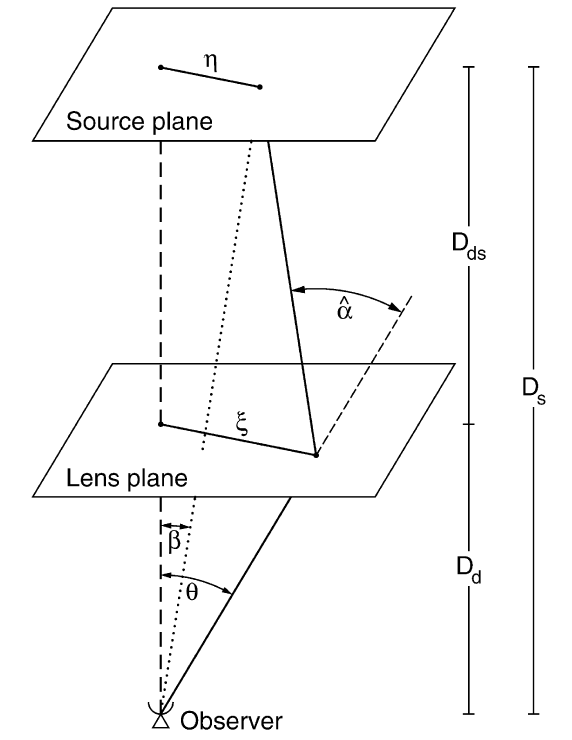
\includegraphics[width=0.5\textwidth]{lensing_figure.png}
	\caption{The sketch of a gravitational lens system created by Michael Sachs,
		under the [CC BY-SA 3.0
	(http://creativecommons.org/licenses/by-sa/3.0) or GFDL
(http://www.gnu.org/copyleft/fdl.html)] license, via Wikimedia Commons.	\label{fig:lens_sketch}
	}
	\end{center}
\end{figure*}
	From General Relativity, we know the gravity of foreground DM creates 
curvature of spacetime, the light emitted by distant galaxies
also follows paths along the curved spacetime, therefore appears {\it
lensed} by the foreground DM distribution. 
 We can write down the surface mass density of the lens
using an integral of along the line-of-sight, i.e. the redshift $z$: 
\begin{equation}
	\Sigma(\vec{\xi}) = \int \rho(\vec{\xi}, z) dz,
\end{equation}
where we use $\vec{\xi}$ to represent a two-dimensional location along the
plane of the lens.
The deflection angle of a light ray at $\vec{\xi}$ can then be represented by
accounting for the deflection at the mass element location
$\vec{\xi}'$:
\begin{equation}
	\hat{\vec{\alpha}} = \frac{4G}{c^2}\int \frac{(\vec{\xi} -
	\vec{\xi}')\Sigma(\vec{\xi}')}{|\vec{\xi} -\vec{\xi}'|} d^2\xi'
= \frac{2}{c^2}\int \vec{\nabla}_\perp \Phi dl.
\end{equation}
where $\Phi$ is the Newtonian gravitational potential.
We can illustrate the deflection in
figure \ref{fig:lens_sketch} to find the relationship between the original
source image and the deflected image:
\begin{equation}
	\vec{\eta} = \frac{D_s}{D_d}\vec{\xi} - D_{ds} \hat{\vec{\alpha}},
\end{equation}
where $D_{ds}, D_d$, and $D_s$ are the various distances indicated in 
Fig. \ref{fig:lens_sketch} respectively.
Substituting the expressions with the angular counterparts:

\begin{align}
	\vec{\beta} &= \vec{\eta} / D_s,\\
	\vec{\theta} &= \vec{\xi} / D_d, \\
	\vec{\alpha}(\vec{\theta}) &=
	\frac{D_{ds}}{D_s}\hat{\vec{\alpha}}(D_d\vec{\theta}),
\end{align}
we can read off each of these quantities (1.4 - 1.6) that appears in the lens
equation from Fig. 1.1:
\begin{equation}
	\vec{\beta} = \vec{\theta} - \vec{\alpha}.
	\label{eq:lens_equation}
\end{equation}


Furthermore, we can first define the effective lensing potential 
$\psi$ which represents a projected Newtonian potential $\Phi$ of the DM lens: 
\begin{equation}
	\psi(\vec{\theta}) = \frac{D_{ds}}{D_d D_s} \frac{2}{c^2} \int \Phi(D_d
	\vec{\theta}, z) dz.
\end{equation}
The reduced deflection angle $\alpha$ also follows:  
\begin{equation}
	\vec{\alpha} = \vec{\nabla}_\theta \psi.
\end{equation}

We can then represent the
distortions of the solid-angle of
the source galaxies in the form of a Jacobian matrix:  
\begin{align}
	\mathbf{A} \equiv \frac{\partial \vec{\beta}}{\partial \vec{\theta}} =
	\frac{\partial (\vec{\theta} - \vec{\alpha})}{\partial \vec{\theta}} =
	\left(
\begin{array}{cc}
1 - \kappa - \gamma_1 & - \gamma_2 \\
- \gamma_2 & 1 - \kappa + \gamma_1
\end{array}
\right),
\end{align}
where $\kappa$ is the dimensionless surface mass density of the lens called the
convergence, and $\gamma_1$ and $\gamma_2$ are the two components of shear.
  
This Jacobian matrix is usually expressed as,  
\begin{align}
\mathbf{A} &= (1 - \kappa)\left(
\begin{array}{cc}
1 - \frac{\gamma_1}{1 - \kappa} & - \frac{\gamma_2}{1 - \kappa} \\
- \frac{\gamma_2}{1 - \kappa} & 1 + \frac{\gamma_1}{1 - \kappa}
\end{array} 
\right) \\
& \equiv (1 - \kappa)\left(
\begin{array}{cc}
1 & 0 \\
0 & 1 
\end{array}
\right)
-
g \left(
\begin{array}{cc}
\cos 2\phi & \sin 2\phi\\
\sin 2\phi & -\cos 2\phi
\end{array}
\right). \label{eq:Jacobian_matrix}
\end{align}
The factor of 2 that exists as part of the phase of the shear, i.e. $\phi$, in
equation (\ref{eq:Jacobian_matrix}) shows 
that galaxy shapes have the properties of a spin-2 field, i.e. showing
a particular kind of rotational symmetry.  In equation 
(\ref{eq:Jacobian_matrix}), it is clear that the convergence is 
responsible for the
isotropic magnification of the light source, while the second term $g$, also
known as the reduced shear, induces changes to the ellipticities of the sources
galaxies. A definition of the convergence is that it
represents the projected surface mass density.
Since the shear is only sensitive to the gradient of the surface
mass density, shear-based techniques can reconstruct $\kappa$ up to a constant.
Physically, this constant can be thought of as a uniform sheet 
of mass in the lens plane and is commonly referred to as the mass-sheet
degeneracy. This degeneracy can be broken if information such as the 
magnification of the
source galaxies is added \citep{Narayan1996}. Another technique for breaking the 
degeneracy requires adding redshift information of individual lensed sources
\citep{Bradac2004}, but may only work for a lens with high enough mass density
within a sizable region. We focus the discussion of lensing analysis techniques
for more general cases when the signal is weak.

Analyzing data in the weak shear limit
(where $\kappa \ll 1$) allows us to approximate the induced shear as $g \approx \gamma$.
This induced shear, however, is a weak signal measured at a $\lesssim 10\%$ 
level of the observed ellipticities for galaxies lensed by galaxy clusters, and
more typically at a $\sim 1\%$ level for cosmic shear \citep{LSSTScienceCollaboration2009}.  
There are other source of contributions to the ellipticity measurements that 
can complicate the inference process. 
Galaxies are generally not round, nor can they all be described by the same 
statistical population. The intrinsic ellipticities of galaxies, also
known as shape noise, is an extra parameter that needs input during the inference.  
Other systematics that can affect ellipticity measurements include 
telescope systematics and atmospheric aberrations.
  To lower the contribution of shape noise,  
one must average the measured ellipticities of the galaxies in the 
same local area of the sky. For these reasons, the local density of source
galaxies limits the measured resolution of the DM
distribution. In chapter 3, I will show how one can
reduce the high-resolution simulated data to match
the weak-lensing resolution based on the source galaxy count.  
In chapter 4, I will elaborate further on the relationship between the 
effective lensing potential $\psi$ with the lensing observables the convergence
and shear for a joint inference.  


\section{Analyzing astronomical data with probabilistic methods}
As our generation of astrophysicists takes on new problems,
we face challenges from observations with 
low signal-to-noise or complicated models with missing variables.
Since astrophysical observations are not controlled experiments, there are limitations 
that cannot be overcome by better experimental designs nor equipment. In
Einstein's words, we need ways to deal with the uncertainties 
when applying mathematical laws to the reality. Breakthroughs in inference 
approaches for extracting scientific information are
therefore crucial for moving our field forward. 
This work describes several attempts to combine astronomical insights
with innovative modeling approaches. This section is dedicated to 
discussing the rationale behind choosing
probabilistic methods for inference, and the corresponding advantages and
disadvantages.

With a Bayesian interpretation of probability, the uncertainty of a random variable 
is expressed using its probability density function \citep{Gelman13}. This
gives a consistent representation of information for sampling and 
hierarchical modeling. Prior information of a system can also be incorporated
through weakly informative priors to achieve faster convergence of the
posterior during sampling. 
While every analysis is based on some assumptions, the
specification of the assumptions through the priors make the process 
transparent for examining the effects of the assumptions.  
A sensitivity analysis that examines how the prior choices
affect the conclusion is presented in chapter 2. 
Other diagnostics for a Bayesian analysis
can be obtained through a posterior predictive check, by generating simulated 
data from the posterior 
distribution to see if they are consistent 
with the observed data. All these diagnostics can help spot any anomaly in
the Bayesian modeling process. Another important advantage of Bayesian
methods is the ease of doing model comparisons by using the Bayes factor (see
chapter 2 for an example).
Formulating the hypothesis correctly is 
otherwise difficult via frequentist statistical tests because 
multiple tests are usually needed to compare more than one dimension of different
multivariate distributions.  

Despite all the listed advantages, Bayesian methods are known to be
computationally slow. A commonly used algorithm, the Metropolis-Hastings Monte 
Carlo Markov Chain (MCMC), only has a theoretical efficiency
(acceptance rate) of $\sim 30\%$ \citep{Roberts97}. A naive implementation of the 
powerful regression algorithm,
the Gaussian Process, also has an $O(n^3)$ computational complexity, where $n$
is the number of galaxies, due to the need
to perform expensive matrix operations. When dealing with precise data,
frequentist methods that make use of summary statistics and estimators show
comparable predictive performance and are often computationally faster. 

To model astrophysical data that has complicated dependencies and significant 
uncertainties, it is more suitable to perform a hierarchical Bayesian inference. 
In chapter 4 of this work, I have provided a graphical model 
to illustrate the hierarchical relationships between variables for the
inference of a DM mass map.
Even though no other detailed graphical model is provided, 
the same line of reasoning is still helpful for 
relating the analyses between chapter 2 and 3.  

\subsection{Reasoning using a Bayesian network}
A probabilistic graphical model (PGM), such as a Bayesian network (BN), 
provides the big picture of a comprehensive scientific analysis. 
While it is possible to come up with an
appropriate set of inference procedures without a graphical model, a graphical
model provides a succinct layout of the relationship between variables.
This is especially important when the number of variables becomes large.
The use of graphical models for inferences in robotics, natural language
processing, and medical diagnosis research have 
shown successes for modeling problems with a high number of variables 
(\citealt{Heckerman1992a}, \citealt{Koller2009}).   

Graphical models can also act as a blueprint for specifying the form of the 
 likelihood function, which is a measure of how good a statistical model fits
the observed data. A BN is represented by a directed acyclic graph (DAG). 
Each of the nodes can take one of the following forms:
\begin{itemize}
		\item a circle represents a random variable  
		\item a shaded circle represents an observed variable
		\item a dot represents a variable with fixed value.
\end{itemize}
An arrow between any two nodes indicates a statistical dependency. 
The direction of the arrow indicates the direction of influence 
of variables, although it is possible for several different graphs to represent 
the same statistical dependencies between variables 
(See Fig. \ref{fig:pgm_examples}).
The direction of the arrows can represent evidential reasoning (or explanation)
when one tries to reason from the observations to the possible causes.
Another line of reasoning, called causal reasoning, can proceed when 
one tries to predict the effects that follow a certain cause.
% All the examples here follow causal reasoning because we understand the
% deterministic physical causes, e.g. cosmology, lensing physics, etc. 
% better than the noisy observations.
The directions of the arrows are therefore not sufficient to determine how the
BN maps to a probability factorization.
The key for interpreting a graphical
model is to find out if dependency-separation exists. 
An proof of dependency-separation and an efficient algorithm for finding 
dependency-separation can be found in \cite{Meek2013} and \cite{Shachter2013}.

\begin{figure*}[h]
	\begin{center}
	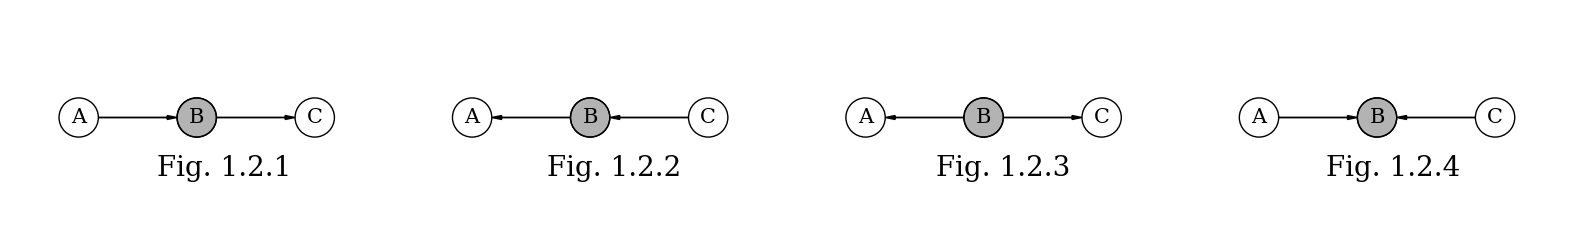
\includegraphics[width=1.\textwidth]{1pt2_pgm_examples.png}
	\caption{
		Similar looking PGMs.	Three of the four PGMs share the same factorization, 
		$P(A, B, C) = P(A | B) P(C | B) P(B)$ (Fig.
		a, b and c) while, Fig. d factors to $P(A, B, C) = P(A, C |
		B) P(B)$. In (a), observing B creates D-separation because B completely
		explains C without A. Similarly, in (b), observing B completely explains A. 
		In (c), B is a confounding factor of A and C that can induce spurious correlation,
		however, observing B, which is the cause of A and C, specifies
		its effect on both A and C, thus removing the correlation between A and C. 
		In (d), A and C both explains B. If B is explained by C
		in a certain way, then A has to explain all the effects that B
		does not explain. There is then induced correlation between A and C that
		needs to be jointly modeled. 
		\label{fig:pgm_examples}
	}
	\end{center}
\end{figure*}

The following toy example can further illustrate how the observation of variables
can affect whether a dependency-separation exists in the graph. 
During a merger between two galaxy subclusters, it is possible to observe an
offset between the DM and the density peak of the member galaxies of the
same subcluster (\citealt{Markevitch2004}, \citealt{Dawson12}, \citealt{Ng2014}), 
which we denote as  $\Delta \vec{s}$. The offset $\Delta \vec{s}$ can depend on both 
the SIDM cross-section $\sigma_{\rm SIDM}$ and other random noise from the 
merger $s_{\rm merger}$. 
Without observing any offset, $\sigma_{\rm SIDM}$ and $s_{\rm merger}$ are
statistically independent. There is no direct arrow between them, they are
d-separated. 

\begin{figure*}[h]
	\begin{center}
	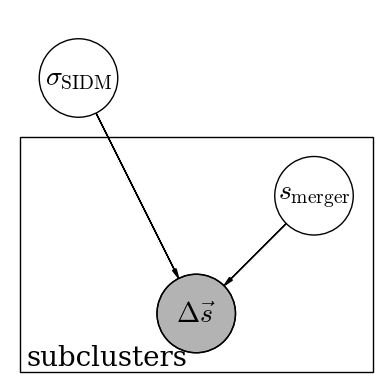
\includegraphics[width=.4\textwidth]{SIDM_pgm.png}
	\caption{PGM explaining what may give rise to a non-zero $\Delta \vec{s}$.
		The plate denotes the part of the PGM that would have different 
		$\Delta \vec{s}$ and $s_{\rm merger}$ for each galaxy cluster (denoted
		with {\it subclusters} in the figure).
		The conditional probabilities corresponding to these nodes inside the plate
		are multiplied together to form the likelihood.
		\label{fig:SIDM_inference}
	}
	\end{center}
\end{figure*}

However, once $\Delta \vec{s}$ is observed, the graph shows a v-structure that
allows the flow of influence between $\sigma_{\rm SIDM}$ and $s_{\rm
merger}$, as both of those two variables are needed to explain the observed
value of $\Delta \vec{s}$. These
statistical dependencies signal the need for a joint inference of 
$\sigma_{\rm SIDM}$ and $s_{\rm merger}$, i.e. one should {\it not} factor
$P(\sigma_{\rm SIDM}, s_{\rm merger} | \Delta
\vec{s}) \approx
P(\sigma_{\rm SIDM} |\Delta \vec{s} ) \times P(s_{\rm merger} |\Delta \vec{s})$
if the goal of the analysis is to infer $\sigma_{\rm SIDM}$.
There have been multiple examples showing how models capturing the conditional 
dependencies have superior fit to the data over models that assume
strong conditional independence (\citealt{Koller2009}). 
Realistically, $s_{\rm merger}$ can be further broken down into a
hierarchical structure that depends on the merger history of the clusters, 
and other properties of the clusters such as the makeup of the population of 
the member galaxies etc. 
Chapter 3 of this work tries to evaluate how these factors may affect $\Delta
\vec{s}$ and whether we can explain the observed values of $\Delta \vec{s}$ 
entirely without a significant $\sigma_{\rm SIDM}$. 
Another application of the graphical model can be
found in chapter 4, where there is an explicit v-structure that guides us to
jointly fit galaxy morphology properties and the Gaussian Process prior.

\begin{figure*}[h]
	\begin{center}
	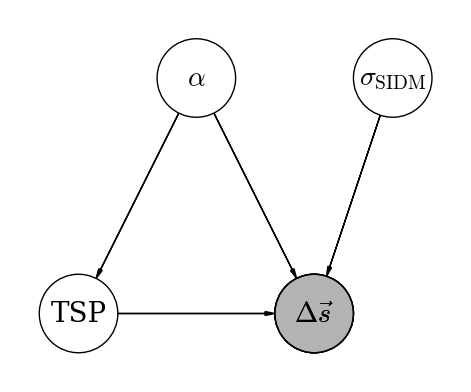
\includegraphics[width=0.4\textwidth]{confounding_alpha_PGM.png}
	\caption{
		Another toy example pertinent to the content in chapter 2. The abbreviated PGM
		shows how the projection angle of the merger axis of
		a galaxy cluster ($\alpha$)	can be an
		unobserved confounding variable that introduces additional correlation between 
		the time-since-pericenter (TSP) and  
		$\Delta \vec{s}$. Since we used a probabilistic
		Monte Carlo approach, the confounding effect is accounted for in Chapter 2.
		\label{fig:confounding_alpha}
	}
	\end{center}
\end{figure*}
There are other advanced uses of graphical models for spotting statistical
dependencies. Graphical models make it easy to spot unobserved confounding
variables that can lead to spurious correlations between other variables (See
Fig.~\ref{fig:confounding_alpha}). A graphical model also makes it clear which 
variables (i.e. the linked neighbor 
nodes) will be affected by the marginalization of a variable. 
There are explicit rules and algorithms about how to change the BN appropriately 
during variable elimination \citep{Murphy2012}. Some of these rules exploits 
the conditional independence of variables to first factor out and marginalize
some disjoint part(s) of the likelihood. After reducing the parameter space to focus
on the interested dimension, the maximization of the likelihood can be sped up.   
  
% reduce the dimensionality of
% the statistical model. Manually inserting latent variable(s) at appropriate
% location(s) of the graphical model can give an approximation of the data variables
% with decoupled statistical dependencies.  
% The approximated statistical independence 
% shows up in the covariance matrix of the variables as entries with very small
% values. This sparsity in the covariance matrix can allow faster optimization of
% the likelihood through sparse matrix inversion techniques.  

Statistical inference is, in general, at least non-deterministic polynomial (NP) 
hard. Verifying scientific hypotheses is usually even more difficult than other
prediction tasks because we cannot simply translate the problem as an 
optimization problem. The scientific hypothesis needs to be formulated 
appropriately in the statistical model. 
This is why I have employed tools such as PGMs to construct physically and 
statistically sound analyses. 


	
% The following commands produce page numbering at the bottom
% center using roman numerals per UC Davis requirements for the
% front matter of the dissertation:
% \pagenumbering{roman}
% \pagestyle{plain}
% The following command produces double-spaced lines for the
% remainder of the document:
\doublespacing
% For some weird reason the counter is offset by 1
\setcounter{chapter}{1}
\chapter{Finding signs of self interacting dark matter in a merging galaxy cluster -
a case study with El Gordo}{}{}

\label{chapter2}
\epigraph{``..., spacetime tells matter how to move''}{John Archibald Wheeler} 

				 
% \cfoot{\thepage}
% \pagenumbering{arabic}

\section{Introduction to merging galaxy clusters} 
Mergers of dark-matter-dominated galaxy clusters probe properties
of the cluster components like no other systems. 
In terms of mass content, dark matter makes up $\sim80\%$ of the mass of clusters
of galaxies, a smaller portion of the mass consist of intercluster
gas($\sim15\%$ in mass content), and sparsely spaced galaxies ($\sim2\%$ in mass content). During a merger of
clusters of the high mass range of $10^{14} M_{\sun}$ to the low mass end of
$10^{15} M_{\sun}$, the subclusters are accelerated to high speeds of 
$\sim 2000 - 3000~\kilo \meter~\second^{-1}$ (\citealt{Lage2014},
\citealt{Dawson12}). The offsets of
different components of the subclusters reflect the differences in the
strengths of interactions between various components. Galaxies are
expected to lead the gas due to their negligible interaction cross
sections with other components. The intracluster medium (ICM) is expected to lose
momentum through electromagnetic interactions. On the other hand, offsets
between dark matter and galaxies may suggest dark matter self-interaction
(\citealt{Kahlhoefer14}, \citealt{Randall2008d}).  
\par
The galaxy cluster ACT-CL J0102-4915, (nicknamed ``El Gordo", at z=0.87),
was discovered via its Sunyaev-Zel'dovich (SZ) effect by the Atacama Cosmology Telescope (ACT;
\citealt{Menanteau2010}; \citealt{Marriage11}); it has the strongest SZ
effect of the full ACT survey \citep{Hasselfield2013}, and was discovered
to be undergoing a major merger approximately in the plane of the sky
(\citealt{M12}, hereafter M12). El Gordo possesses a range of noteworthy features that allow us to constrain the merger dynamics in multiple ways. 
\begin{figure*}
	\includegraphics[width=1\textwidth]{ElGordo.pdf}
	\caption{Configuration of El Gordo showing overlay of dark
		matter distribution in blue, and X-ray emission in red. 
		(Image credit: NASA, ESA and \citealt{Jee13}). 
		The cross markers show the positions of the northwest (NW) and
		southeast (SE) dark matter density peaks, and the center of mass (CM)
		locations respectively. Note that the mass ratio of the NW subcluster
		to the SE subcluster is $\sim 2:1$ \citep{Jee13}. 
		The dashed white lines indicate the approximate location and extent of the northwest radio relic (NW relic), the east radio relic (E relic) and the
		southeast radio relic (SE relic) \citep{L13}.
		\label{fig:config}
	}
\end{figure*}
From the spectroscopy and Dressler-Schectman test for the member galaxies
in \cite{Sifon13}, it is shown that El Gordo does not have complicated
substructures in its galaxy velocity distribution. 
El Gordo is further confirmed to be a binary merger 
from the weak lensing analysis by \cite{Jee13}. The weak lensing analysis shows
a mass ratio of $\sim$2:1  between the two main subclusters, named
according to their location as the northwest (NW) and southeast (SE) subclusters respectively 
(See Figure~\ref{fig:config}). A bimodal distribution of cluster member galaxies is
also observed \citep{M12}. In addition, El Gordo has an interesting X-ray morphology. In the northwest, it shows a wake feature, i.e.,
turbulent flow due to object of higher density moving through fluids, while
in the southeast, it shows the highest X-ray emissivity indicative of a
cool gas core at the head of the wake. The most straightforward explanation for this morphology is that the
cool gas core has passed from the northwest to the southeast
\citep{M12}. 
The high mass of El Gordo also makes it a good
gravitational lens. \cite{Zitrin13} have found multiple strong
gravitationally lensed images around the center region of El Gordo. 
On the outskirts, strong radio emission is detected in
the NW and the SE respectively. These radio emitting regions show steep spectral
index gradients and are identified as radio relics associated with shock waves
created from the merger \citep{L13}. El Gordo is one of $\sim 50$ galaxy clusters that have
been associated with a radio relic and show dissociation between the X-ray
gas and the DM subclusters. \par 

\begin{figure*}
	\includegraphics[width=\linewidth]{merger_cartoon_white_bg.pdf}
	\caption{Illustration of the spatial location of different components of El Gordo at
		different stages of the merger. Earlier stages (with a smaller TSP) are on the left side of later stages. The rightmost returning scenario is preferred from our simulation.} 
	\label{fig:merger_cartoon}
\end{figure*}
In this paper, we combined most of the available information of El Gordo
with the main goal of giving estimates of
the dynamical parameters after taking into account all
constraints and uncertainties due to the missing variables.
Since mergers of clusters proceed on the time-scale of many millions of
years, one of the most important missing variables to infer is the
time-since-pericenter (TSP)$^\dagger$, which is defined to be the time when the mass
peaks of the DM subclusters are at minimum separation. \footnote{TSP in this
	paper is completely identical to the variable time-since-collision (TSC) in
	\cite{Dawson12}. We have renamed the variable to avoid confusion about how we
define collision as pericenter.}
Determining the TSP of similar clusters helps
us reconstruct different stages and recover the physics of a cluster merger.
In particular there is a degeneracy between the following two possible
scenarios:
We call the scenario for which the subclusters are
moving apart after pericenter to be ``outgoing", and the alternative scenario 
``returning" for which the subclusters are approaching each other after turning
around from the apocenter for the first time (See
Fig.~\ref{fig:merger_cartoon}).\par
Another crucial, missing piece of information is the 3D
configuration, i.e.\ the angle between the plane of the sky and the merger
axis called the projection angle $\alpha$. Since most of the dynamical
observables are projected quantities while the modelling of physics
requires 3D
variables, the deprojection contributes the
largest amount of uncertainty to the dynamical variables
(\citealt{D13}, hereafter D13). The morphology of the double relic of El Gordo suggests that
$\alpha$ should be small. 
For mergers with a
large projection angle, the radio emission would be projected towards the
center of the merger, which inhibits detection \citep{Vazza11}.
However, the only quantitative constraint on $\alpha$ for El Gordo is from
the analysis of the radio relic from \cite{L13} with a lower bound of $\alpha \geq 11.6 \degree$. A tighter
constraint on $\alpha$ is needed for us to reduce uncertainty of the
dynamical variables. 
\par 
We employed a data-driven approach that thoroughly probes parameter
space by directly drawing samples from the probability density functions
(PDFs) of
the observables. 
This work based on Monte Carlo simulation is particularly important since
the phase space of possible merger scenarios is large. Previous attempts at modeling El Gordo with hydrodynamical
simulations such as \cite{Donnert13} and \cite{Molnar14} provided only in
total a dozen possible configurations of El Gordo, which do not
reflect the range of input uncertainties. Another approach for
estimating dynamical parameters would be to look for multiple analogs of El Gordo in cosmological
simulations.  However, under the hierarchical picture
of structure formation in the $\Lambda$CDM model, there is a rare chance
for massive clusters like El Gordo to have formed at a redshift of $z = 0.87$.  
The number density of analogs with mass comparable to El Gordo in a
cosmological simulation is as low as $10^{-11} \mega\text{pc}^{-3}$
\citepalias{M12}.\par
In the following sections, we adopt the following conventions: (1) we
assume the standard $\Lambda$CDM cosmology with $\Omega_{m} = 0.3$,
$\Omega_{\Lambda} = 0.7$ and $H_0 = 70~\kilo\meter / \second / \mega
{\rm pc}$. (2) All confidence intervals are quoted at the 68\% level unless otherwise stated. 
(3) All quoted masses ($M_{200c}$) are based on mass contained
within $r_{200}$ where the mass density is 200 times the critical density
of the universe at the cluster redshift of $z = 0.87$. 
\begin{figure}
	\includegraphics[width = \linewidth]{confirmed_member_divide.png}
	\caption{\label{fig:membership} Points showing the locations of the
	member galaxies and the division of the member galaxies among the two subclusters of El Gordo by a spatial cut
(black line). The color of the points shows the corresponding spectroscopic
redshift of the member galaxies (see color bar for matching of
spectroscopic values), with the redder end indicating higher
redshift. The galaxy number density contours in the background in green indicate a bimodal
distribution.} 
\end{figure}
\section{Data} 
We gathered and analyzed data from multiple sources. 
See Table~\ref{tab:inputs} for descriptions of the PDFs of the input
variables. 
We examined the
spectroscopic data obtained from the Very Large Telescope (VLT) as described in \citetalias{M12} and \citet{Sifon13} for estimating the
relative velocity differences between the subclusters.
We adopted the identification of galaxy membership of El Gordo given by
\citet{Sifon13} with a total count of 89 galaxies.
To further distinguish member galaxies of each subcluster, we adopted the
spatial cut from \citetalias{M12}.
The adopted spatial cut is approximately perpendicular to the 2D merger
axis \citepalias{M12} and is consistent with
the bimodal number density contours (See Fig.~\ref{fig:membership}). 
There are 51 members identified in the NW subcluster and 35 members in the SE
subcluster. \par 
For the weak-lensing mass estimation, we used the
Monte Carlo Markov Chains (MCMC) mass estimates from \citetalias{Jee13}.
The Hubble Space Telescope data used in \citetalias{Jee13} were obtained from two
programs PROP 12755 and PROP 12477. PROP 12755 consisted of two pointings in the F625W, F775W, and F850LP.
F850LP for a 6' x 3' strip, while PROP 12477 provided a $2 \times 2$ mosaic
pattern with F606W and a single pointing in F814W. 
\par 
In order to further constrain our parameter space, we referred to the properties of
the radio relics from \citet{L13}. El Gordo shows radio emission on the
periphery of both subclusters \citepalias{M12}. The two radio relics, the
northwest (NW) relic and the southeast (SE) relic, of El Gordo were
tentatively identified
in the Sydney University Molonglo Sky Survey (SUMSS) data in low
resolution at 843 MHz \citep{Mauch03} as shown in M12. Higher
resolution radio observations conducted by \cite{L13} at 610 \mega Hz and
2.1 \giga Hz later confirmed the identities of the NW and the SE relic, and
found another extended source of radio relic in the east (E) (See Fig.~\ref{fig:config}). Among the radio relics, the NW relic possesses the most extended geometry
(0.56 Mpc in length), and its physics, including the
polarization and Mach number, were studied in the greatest detail. Such
information allows us to constrain $\alpha$ and the merger scenario. The E relic
was also reported to have a resolved length of 0.27 Mpc, while the SE relic
was found to overlap with a point source \citep{L13}. Both the E and SE
relic are closer to the SE DM subcluster, so we considered them to
originate from the same merger shock in the following work.
\section{Method -- Monte Carlo simulation} 
\label{sec:method}
We used the collisionless 
dark-matter-only Monte Carlo modeling code written by \citetalias{D13}, to
model the dynamics of the DM subclusters of their first core-passage.
In the D13 code, the time evolution of the
head-on merger was computed based on an analytical, dissipationless model
assuming that the only dominant force is the gravitational attraction from
the masses of two Navarro-Frenk-White (hereafter NFW) DM halos
\citep{Navarro96}. 
The gravitational attraction was evaluated and summed at 10 000 fixed grid
points of each of the analytic NFW halo profiles out to the respective
$r_{200c}$.\par
In the simulation, many realizations of the collision are
computed by drawing random realizations of the PDFs of the inputs. Most
input variables are obtained from previous observations ($\vec{D}$).  One
unknown model variable, which is the projection angle between the plane of the sky
and the merger axis, $\alpha$, is drawn from the PDF of $\alpha$ being
observed: 
\begin{equation}
	\alpha^{(j)} \sim f(\alpha) = \cos \alpha.
\end{equation}
and the calculation of the output variables of the $j$-th realization can be denoted as: 
\begin{equation}
	(\vec{\theta}^\prime)^{(j)} = g(\alpha^{(j)}, \vec{D}^{(j)}), 
\end{equation}    
for a suitable function $g$ that describes conservation of energy during
the collision of the two NFW halos due to the mutual gravitational
attraction.  In particular, the required $\vec{D}$ includes the masses ($M_{200_{NW}},M_{200_{SE}}$) the redshifts ($z_{NW}, z_{SE}$) and the
projected separation of the two subclusters ($d_{\rm proj}$).  See
Table~\ref{tab:inputs} for quantitative descriptions of the sample PDFs, and
the outputs with physical importance are described in detail in Section~\ref{sec:outputs}. \par
Finally, we excluded realizations that produce any unphysical output
values, such as realizations with time-since-pericenter larger than the age of universe at the
cluster redshift.  We refer to this process of excluding unphysical
realizations as applying weights. 
To ensure convergence of the output PDFs, in total, 2 million realizations
were computed. However, the estimates would agree up to 1\% just 
from 20 000 runs \citepalias{D13}. 
Even though we describe the weights for one variable at a time 
(See Appendix~\ref{app:priors}), 
the correlations between different variables are properly taken into account
since we discarded all the variables of the problematic
realizations.\par 
\begin{table}
	\caption{Properties of the input sampling PDFs ($\vec{D}$) of the Monte Carlo
simulation. We obtained estimates of the inputs via different methods. $^a$We
made used of the MCMC chains from \citetalias{Jee13} for mass-related
estimates (See Section \ref{subsubsec:WL_mass_estimate}
). $^b$The redshift distributions were obtained from bootstrapping (See Section 
\ref{subsubsec:membership_and_redshift}).
$^c$We approximated the positions of the centroids with 2D Gaussians before we
calculated the projected separations of the subclusters (See Section 
\ref{subsubsec:proj_sep}). Even though the distributions of the mass estimates 
and the redshift were not estimated via parametric methods (e.g. fitting mean
and variances of Gaussians), they
resemble Gaussian distributions due to the Central Limit Theorem.
} 
\begin{center} 
\begin{tabular}{@{}lccccc}
\hline \hline Data & Units & Location & Scale & Ref \\ \hline
$M_{200c_{\mathrm{NW}}}$ & $10^{14} h_{70}^{-1}$ M$_{\odot}$ &13.0&1.6&
\citetalias{Jee13}$^a$\\ 
c$_{\mathrm{NW}}$ &  & 2.50& 0.02& \citetalias{{Jee13}}$^a$ \\ 
$M_{200c_{\mathrm{SE}}}$ & $10^{14} h_{70}^{-1}$ M$_{\odot}$ &7.6&1.2 &
\citetalias{Jee13}$^a$\\ 
$c_{\mathrm{SE}}$ &  & 2.70 & 0.04& \citetalias{Jee13}$^a$\\ 
$z_{\mathrm{NW}}$ &  & 0.86842 & 0.00109& \citetalias{M12}$^b$\\ 
$z_{\mathrm{SE}}$ &  & 0.87110 & 0.00117& \citetalias{M12}$^b$\\ 
d$_{\mathrm{proj}}$ & Mpc & 0.74 &0.007 & \citetalias{Jee13}$^c$\\ 
\hline 
\end{tabular} 
\end{center} 
\label{tab:inputs} 
\end{table} 
The system of El Gordo satisfies several major assumptions in the Monte Carlo
simulation. One of the strongest assumptions is that all realizations correspond to
gravitationally bound systems. The simulation excludes all realizations
that would result in relative pericenter velocities of the subclusters
higher than the free-fall velocity. We justify our assumption of
modeling only gravitationally bound systems by noting that the relative escape
velocity of the subclusters for El Gordo is
$4500~\kilo\meter~\second^{-1}$ (based on the mass estimates of
\cite{Jee13}). Studies from cosmological simulations giving the PDFs of the pairwise
velocities of massive merging clusters ($>10^{15} M_{\sun}$) indicate that it
is highly unlikely that the pairwise velocities would be $> 3000~\kilo
\meter~\second^{-1}$ under $\Lambda$CDM (\citealt{Thompson12},
\citealt{Lee2010}).\par
Other major assumptions for modeling systems with this code include negligible impact parameter.
Several papers have noted that the X-ray morphology of a bimodal merger is
sensitive to the impact parameter (\citealt{Springel2007},
\citealt{Ricker98}, \citealt{Mastropietro2008a}); an impact
parameter as small as 0.1 Mpc can result in substantial asymmetry. 
The X-ray morphology of El Gordo is approximately symmetric about the merger axis. 
On the other hand, the dynamics of the merger is not as sensitive to the
impact parameter as the X-ray morphology. The simulations of
\cite{Ricker98} of bimodal mergers of $10^{15} M_{\sun}$ halos, showed that the
resulting relative velocity would be approximately $2000 \text{ km s}^{-1}$, relatively
insensitive to impact parameters between 0 to 5 times the scale radius ($5~r_s = 3.5$ Mpc). \cite{Mastropietro2008a} also reported that
an impact parameter of $0.1~r_{200} = 0.14$ Mpc affected merger dynamics only
at the $\sim$10\% level. \citealt{Molnar14} indicated that the impact parameter of El Gordo
may be as large as $40\%~r_s \approx 0.3$ Mpc, where $r_s$ is
the corresponding characteristic core
radius of the NFW halo with the mass of the SE subcluster. We attribute
the result from \citealt{Molnar14} to incomplete exploration of
the parameter space, and note that other impact parameter values may also match the
X-ray observables of El Gordo. \par
Other assumptions in this simulation include negligible dynamical friction
during the merger, negligible mass accretion and negligible self-interaction
of dark matter. Discussion of the effects of each of these assumptions is
included in \citetalias{D13}.  
\subsection{Inputs of the Monte Carlo simulation} \label{sec:inputs}
\subsubsection{Membership selection and redshift estimation of subclusters}
\label{subsubsec:membership_and_redshift}
After identifying members of each subcluster, 
we performed 10, 000 bootstrap realizations to estimate the biweight
locations of the spectroscopic redshifts of the respective members in order
to obtain the samples of the PDFs of the redshifts of each subcluster. 
The spectroscopic redshift of the subclusters were
determined to be 
$z_{\mathrm{NW}} = 0.86842 \pm 0.0011$ and 
$z_{\mathrm{SE}} = 0.87131 \pm 0.0012$, where the quoted numbers represent the
biweight location and 1$\sigma$ bias-corrected confidence level
respectively \citep{Beers90}.  
Both the estimated redshifts of the subclusters and the uncertainties are
consistent with estimates of $z=0.8701 \pm 0.0009$ for El Gordo given by 
\citealt{Sifon13}, and the fact that the
member galaxies of El
Gordo shows large velocity dispersion, i.e.\ the largest velocity
dispersion among all the ACT galaxy clusters, as reported by
\citetalias{M12}.
\begin{figure}
	\includegraphics[width = \linewidth]{bootstrapped_redshift.png}
	\caption{Bootstrapped location of the
	redshift estimates and $v_{rad}$ estimates for each subcluster using the
	selected spectroscopic members. The shaded histograms represent the
	bootstrapped samples.
} \label{fig:bootstrap_redshift}
\end{figure}
We estimated the radial velocity differences of the
subclusters by first calculating the velocity of each subcluster with
respect to us, using  
\begin{equation}
	v_i = \left[ \frac{(1+z_i)^2 - 1 }{(1+z_i)^2 + 1 }\right]c,
\end{equation}
where $i=1, 2$ represents the two subclusters, and $c$ is the speed of
light. The relative radial velocity was calculated by: 
\begin{equation}
	\Delta v_{rad}(t_{obs}) = \frac{|v_2 - v_1|}{1-\frac{v_1 v_2}{c^2}}.
\end{equation}
We obtained a low radial velocity difference of the two subclusters to be
$476~\pm~242~\kilo\meter~\second^{-1}$ (See Fig.~\ref{fig:bootstrap_redshift}). 
The radial velocity difference of $586~\kilo \meter~\second^{-1}$ reported by \citetalias{M12} 
is higher than our estimates but within the 68\% bias-corrected
confidence interval.\footnote{bias from the location estimator of
	the bootstrapped distribution not giving the maximum likelihood value was
corrected for.} 
% Limitations and possible improvements of this analysis
% of $v_{rad}$ are provided in the discussion. 
\subsubsection{Weak lensing mass estimation} 
\label{subsubsec:WL_mass_estimate}
We obtained 40, 000 samples of the joint PDFs of the masses of the two dark
matter halos as the outputs of the Monte Carlo Markov Chain (MCMC)
procedure from \citealt{Jee13}. Discussion of the handling of the weak
lensing source galaxies and the details of the MCMC procedure for mass
estimation can be found in \citealt{Jee13}. 
\subsubsection{Estimation of projected separation ($d_{\rm proj}$)} 
\label{subsubsec:proj_sep}
To be consistent with our MCMC mass inference, our Monte Carlo simulation takes 
the projected separation of the NFW halos to be those of the inferred
DM centroid locations in \citealt{Jee13}. We drew random samples
 of the location of centroids from two 2D Gaussians centered at
 R.A.$=$01:02:50.601, Decl.=$-$49:15:04.48 for the NW subcluster and R.A. =
 01:02:56.312, Decl.=$-$49:16:23.15 for the SE
subcluster, with a 1'' standard deviation each as estimated from the
convergence map of \citet{Jee13}. The
inferred centroid locations correspond to a mean projected separation
($d_{\rm proj}$) of $0.74\pm {0.007}$ Mpc.  
\subsection{Outputs of the Monte Carlo simulation}\label{sec:outputs}
We outline the outputs of the simulation here to facilitate the discussion
of the design of the weights used in the simulation. The simulation
provides PDF estimates for 8 output variables. Variables
of the highest interest include the time-since-pericenter and the angle $\alpha$, which is
defined to be the projection angle between the plane of the sky and the
merger axis. Other output variables are dependent on $\alpha$ and time. Specifically, the simulation denotes the time dependence by
providing several characteristic time-scales, including the time
elapsed between consecutive collisions
($T$) and the time-since-pericenter of the observed state ($TSP$), with the
time of pericenter defined to be when the centers of the two NFW halos coincide. 
\par
We provide two versions of the time-since-pericenter variables $TSP_{\rm out}$ and
$TSP_{\rm ret}$ to denote different possible merger scenarios. 
1) The TSP for the``outgoing" scenario corresponds to the
smaller $TSP_{\rm out}$ value, and 2) the ``returning'' scenario 
corresponds to the larger $TSP_{\rm ret}$.
We describe how we make use of properties of the radio relic to evaluate
which scenario is more likely in
section~\ref{sec:positionprior}. Evolution of the merger after the second
passage is not considered. Outputs from our dissipationless simulation for
a ``second'' passage will not differ from the first passage, and the
predicted relic position would be so far for us to rule this out.
 
The simulation also outputs estimates of variables that describe
the dynamics and the characteristic distances of the merger. The relative
3D velocities of the subclusters, both at the time of the
pericenter ($v_{3D}(t_{\rm per})$) and at the time of observation
($v_{3D}(t_{obs})$) are provided. The characteristic
distances included in the outputs are the maximum 3D separation ($d_{max}$),
which is the distance between the subclusters at
the apocenter and the 3D separation of the subclusters at observation
($d_{3D}$). 
\subsection{Design and application of weights} 
\label{sec:priors}
One of the strengths of the Monte Carlo simulation by
\citetalias{D13} is its ability to detect and rule out extreme input values that would result in
unphysical realizations via the application of weights. 
Our default weights are described in D13 and we include them in
Appendix~\ref{app:results} for the convenience of the readers. 
In addition, we have devised a new type of weights of the projection angle $\alpha$
based on the polarization fraction of the radio relic.

%---------------------------------------------------------------------------

\subsubsection{Monte Carlo weights based on the polarization fraction of the radio relic}
\label{subsubsec:polar_frac}

We can relate the polarization fraction of the radio relic to the
projection angle by examining the
generating mechanism of the radio relic.
The observed radio relic was generated by synchrotron emission of free electrons in a
magnetic field. If the magnetic field was uniform, the observed
polarization fraction of the synchrotron emission of the electrons depends on the
viewing angle (or equivalently the projection angle) with respect to the
alignment of the magnetic field. Synchrotron emission from electrons inside
unorganized magnetic field is
randomly polarized. The high reported integrated polarization fraction from
\citet{L13} can be explained by a highly aligned magnetic field,
compressed along with the ICM during a merger
(\citealt{E98}, \citealt{vanWeeren10}, \citealt{Feretti12}).
%This picture is consistent with a high polarization fraction.
\par

We designed the weights to reflect how $\alpha$ decreases monotonically as the
maximum observable integrated polarization fraction ($\langle P \rangle$). 
\begin{figure}
	\includegraphics[width=\linewidth]{Ensslin_polar_fig.png}
	\caption{Predictions of polarization percentage of the radio relic at a
		given projection angle from different models, reproduced from
		\citep{E98} or equation~\ref{eqn:Ensslin_model}. Each model assumes electrons producing the radio emission
		to be accelerated inside uniform magnetic field of various strengths ({\it strong} or 
		{\it weak}). The curves are plotted with spectral index of the radio emission
		($\alpha_{radio}$), spectral index of the electrons ($\gamma$) and
		compression ratio of the magnetic field ($R$) corresponding to the
		estimated values from \citet{L13}.
		We highlight the observed polarization percentage of the main NW radio relic
		of El Gordo by the dotted vertical line with the greyed out region
		indicating the uncertainty \citep{L13}.\label{fig:Ensslin_fig}}
\end{figure}
This assumption is based on the class of models given by \cite{E98}(See
Figure~\ref{fig:Ensslin_fig}). In particular, we refer to a model from \cite{E98} 
that would give the most
conservative estimate on the upper bound of $\alpha$:
\begin{equation}
	\alpha = 90 \degree - \arcsin \left( \sqrt{\frac{\frac{2}{15} \frac{13R -
	7}{R - 1} \frac{\gamma + 7/3}{\gamma + 1} \langle P_{strong} \rangle}{1 +
		\frac{\gamma + 7/3}{\gamma +1} \langle P_{strong} \rangle
	}}\right),\label{eqn:Ensslin_model}
\end{equation}
This model corresponds to the case of a strong field with the relic being supported by
magnetic pressure only, with the spectral index of the radio
emission being $\alpha_{radio} = 0.86$, the compression ratio of the
magnetic field being
$R=2.7$ and the spectral index of the electrons being $\gamma = 2.7$
\citep{L13}. 
This model predicts a maximum integrated polarization fraction 
 of
$\sim60\%$ when $\alpha \rightarrow 0$. 
%We consider 39\degree as an upper bound on the projection angle since this 
% idealized model assume isotropic distribution of magnetic field and
%electrons. 
This  polarization fraction of $\sim60\%$ predicted by \citep{E98} is
consistent with the upper bound of relic polarization fraction in cosmological
simulations \citep{S13}. From this model, the
observed integrated polarization fraction of $33\%\pm1\%$ corresponds to an estimated value
of $\alpha  = 35\degree$. 
No other model of the magnetic field should predict 
a higher polarization fraction, thus it is highly unlikely that we see 33\%
integrated polarization at $\alpha > 35\degree$.  
\par

We cannot rule out $\alpha \leq 35\degree$ because magnetic field
nonuniformities can lower the polarization below the Ensslin model value.
\cite{E98} assumes an isotropic distribution of electrons in an isotropic magnetic field. Cosmological
simulations of radio relics from \cite{S13} show varying polarization
fraction across and along the relic assuming $\alpha = 0$, resulting in a
lower integrated polarization fraction. For example, it is possible to see 
an edge-on radio relic ($\alpha = 0$) with integrated polarization fraction of 33\%. 
Furthermore, \cite{S13} shows that after convolving the
simulated polarization signal with a Gaussian kernel of 4\arcmin~to
illustrate effects of non-zero beam size, the polarization fraction drops
to between 30\% to 65\% even when $\alpha = 0$. We examined the effects of perturbing
the cutoff value of this weight to ensure the uncertainties do not
introduce significant bias in the estimated output variables in
section~\ref{sec:sensitivityTests}.
To summarize, we used a conservative uniform weight to encapsulate the
information from the polarization fraction of the radio relic as:
\begin{equation}
w(\alpha) = 
	\begin{cases}
	& \text{const. for  }\alpha < 35 \degree \\ 
	& 0 \text{ otherwise,}\label{eqn:polarprior}.
	\end{cases}
\end{equation}
We refer to equation~\ref{eqn:polarprior} as the polarization weights. Unless
otherwise stated, the main results of the paper are obtained after applying
this polarization weight in addition to the default weights.

%%---------------------------------------------------------------------------

\subsection{Extension to the Monte Carlo simulation - Determining merger
scenario with radio relic position by model comparison}
\begin{landscape}
\begin{table*}
	\caption{List of variables that provide quantitative constraints for the merger
		scenario. For details of the distribution of each variable see the corresponding
	$^\dagger$Section. Calculations were done with all available realizations
instead of the best estimate value listed here.}
\begin{center} 
\begin{tabular}{@{}lccccc}
	\hline \hline Variable & Best estimate value & Unit & Section$^{\dagger}$ \\ 
	\hline
Time averaged speed of SE relic in the CM frame ($\langle v_{relic} \rangle$) 
& 530 &  km~s$^{-1}$  & \ref{sec:merger_scenario}\\
Time averaged speed of NW relic in the CM frame ($\langle v_{relic} \rangle$) &
	310 &  km~s$^{-1} $ & \ref{sec:merger_scenario}\\
Projected separation of SE relic from the CM ($s_{proj}$)  & 1.1  & Mpc & \ref{sec:positionprior} \\ 
Projected separation of NW relic from the CM ($s_{proj}$)  & 0.63 & Mpc & \ref{sec:positionprior} \\ 
Outgoing time-since-pericenter ($TSP_{out}$)  &  0.61 & Gyr &
\ref{sec:outputs}, 
\ref{sec:merger_scenario}
\\ 
Returning time-since-pericenter ($TSP_{ret}$)  & 1.0 & Gyr & \ref{sec:outputs}, 
\ref{sec:merger_scenario}
\\ 
Age of the universe at z = 0.87 & 6.30 & Gyr&  \\ 
Free fall velocity of subclusters & 4500 & km~s$^{-1}$ & \ref{sec:method}\\  
Polarization fraction of NW relic ($\langle P_{strong} \rangle$) & 33\% &  &
\ref{subsubsec:polar_frac}\\ 
\hline 
\end{tabular} 
\end{center} 
\label{tab:input_contraints} 
\end{table*} 
\end{landscape}

One of the biggest questions involving the merger is whether El Gordo is
observed during a returning or outgoing phase. We compared the two merger
scenarios by making use of the observed projected separation of the relic from the
center of mass.
Simulations of cluster mergers such as the work of \citet{Paul2011b},
\citet{VanWeerenRJ2011}, and \citet{Springel2007} showed that merger shock
fronts that may correspond to the radio relics 1) are generated near the
center of mass of the subclusters close to the time of the first
core-passage, 2) propagate outward with the shock speed decreasing only slightly.
The propagation speed of the shock wave {\it with respect to the
center-of-mass} is reported 
to drop between $\sim 10\%$ from \citet{Springel2007} and  
10\% to 30\% from \citet{Paul2011b} (note that the   
 time resolution is 0.6 Gyr for the simulation in \citealt{Paul2011b}).
\par 
To capture the monotonically decreasing trend of the
propagation speed of the shock fronts with respect to the center of
mass, we expressed the possible time-averaged shock speeds as a factor of the inferred
pericenter speed of the corresponding subcluster in the center of mass
 frame. 
Then we calculated how far the shock would have propagated for our inferred
$TSP_{\rm out}$ and $TSP_{\rm ret}$ values. We worked in the center of mass frame where the
shock speed is expected to drop slightly with TSP. 
The projected separation of the shock is approximated as:
\begin{equation}
	%s_{proj} = \langle v_{relic} \rangle (\hat{t}_{obs} - \hat{t}_{col})
	s^j_{proj} \approx \langle v_{relic} \rangle^j (t^j_{obs} - t^j_{per})
	\cos(\alpha^j),
	\label{eq:proj_s_model}
\end{equation}
where the superscript $j$ of any variable denotes the value of the
variable from the j-th realization of the simulation, and $s_{proj}$ is the estimated projected
separation. We estimated the upper and lower bounds of the time-averaged velocity
$\langle v_{relic} \rangle$ of the shock between
the pericenter of the subclusters and the observed time as:  
\begin{align}
	\label{eqn:NW_speed}
	\langle v_{NW relic} \rangle^j &= \beta~v^j_{3D, NW}(t_{\rm per}) \\
	&= \beta~v^j_{3D}(t_{\rm per}) \frac{m^j_{SE}}{m^j_{SE} + m^j_{NW}}, 
\end{align}
where  $\beta$ is a factor that we introduce to represent the
uncertainty of the velocity of the relic shock wave, $v_{3D, NW}(t_{\rm per})$ 
refers to the pericenter velocity of
the NW subcluster in the center-of-mass frame as a comparison, and $m$
represents the mass within $r_{200c}$ of each subcluster as denoted by the
labels in the subscripts. 
Likewise, we have also computed the expected projected separation of the SE
relic using:  
\begin{equation}
	\label{eqn:SE_speed}
	\langle v_{SE relic} \rangle^j = \beta~v^j_{3D}(t_{\rm per}) \frac{m^j_{NW}}{m^j_{SE} + m^j_{NW}}. 
\end{equation}
\par 
\begin{figure}
	\includegraphics[width=\linewidth]{TwoMnWBSG_2contour2d.png}
	\caption{The marginalized output PDF of the returning time-since-pericenter
($TSP_{\rm ret}$) vs. the 3D velocity at the time of pericenter for El Gordo. The
grey set of contours show the confidence regions before applying the
polarization weight and the colored contours correspond to the confidence
regions after applying the weights. The contours represent the 95\% and
68\% confidence regions respectively. }
	\label{fig:TSP_v3D}
\end{figure}

\begin{landscape}
\begin{table*}
\caption{Table of the output PDF properties of the model variables and output variables from Monte Carlo simulation
\label{tab:outputs}}
\begin{tabularx}{\textwidth}{@{\extracolsep{\fill}}lccccccccc@{}}
\cmidrule{1-10}     
&&&&Default weights & & & & Default + polarization weights  \\ 
\cmidrule{4-6} \cmidrule{8-10} 
Variables & Units && Location & 68$\%$ CI $^{\dagger}$ &95$\%$ CI && Location & 68$\%$ CI  & 95$\%$ CI \\ 
\cmidrule{1-10}     
$\alpha$ &(degree)&&43&19-69&6-80&&21&10-30&3-34\\
$d_{\rm proj}$ &Mpc&&0.74&0.74-0.75&0.73-0.76&&0.74&0.74-0.75&0.73-0.76\\
$d_{\rm max}$ &Mpc&&1.2&0.90-2.2&0.77-4.6&&0.93&0.81-1.2&0.75-1.9\\
$d_{\rm 3D}$ &Mpc&&1.0&0.79-2.1&0.75-4.3&&0.80&0.76-0.88&0.74-0.91\\
$TSP_{\rm out}$&Gyr&&0.61&0.4-0.95&0.26-2.4&&0.46&0.30-0.55&0.21-0.64\\
$TSP_{\rm ret}$&Gyr&&1.0&0.77-1.7&0.63-4.4&&0.91&0.69-1.3&0.59-2.3\\
$T$&Gyr&&1.6&1.3-2.4&1.2-6.4&&1.4&1.2-1.6&1.2-2.2\\
$v_{\rm 3D}(t_{\rm obs})$ & \kilo \meter~\second$^{-1}$ &&580&260-1200&59-2400&&940&360-1800&62-2900\\
$v_{\rm rad}(t_{\rm obs})$ & \kilo \meter~\second$^{-1}$ &&360&140-630&27-880&&310&110-590&8-840\\
$v_{\rm 3D}(t_{\rm per})$ & \kilo \meter~\second$^{-1}$ &&2800&2400-3700&2100-4200&&2400&2200-2800&2100-3500\\
\cmidrule{1-10}    
\end{tabularx}\\
\footnotesize{$\dagger$ CI stands for confidence interval}\\
\end{table*}
\end{landscape}

For the most likely range of $\beta$, we refer to the
simulations of cluster mergers by both \cite{Springel2007} and
\cite{Paul2011b} because those are some of the few simulations available that
quote shock propagation speeds in the center-of-mass frame of the cluster,
rather than the ICM frame. 
The simulation of the Bullet Cluster by \cite{Springel2007}, 
indicates that the propagation velocity of the shock evolves such that $\beta \approx 0.95$ within
$\sim 0.4~\giga$yr after the pericenter. For the analysis of El Gordo,
we suggest $\beta \approx 0.9$ to be the most likely value given that the $TSP$ of
El Gordo is longer. 
To include the possible range of valid $\beta$ values,
we examined $0.7 \leq \beta \leq 1.5$. This range of $\beta \approx 1$ allows us to use  
equations~\ref{eqn:NW_speed} and~\ref{eqn:SE_speed} to reflect that the
shock is driven by the merger. We note that the propagation speed of the
shock is also determined by the temperature, density and other details of
the gas medium (\citealt{Prokhorov2007}, \citealt{Springel2007},
\citealt{Milosavljevic07}), so it is physically possible for the shock to
propagate with $\beta > 1$. An example of
merging clusters (Merger F) with $\beta \approx 2.0$ has been reported by the cosmological
simulations in \citealt{Paul2011b}. 
However, we note that Merger F from \citealt{Paul2011b} has a lower mass of
$\sim 1.1 \times 10^{14} M_{\sun}$ in total, and that the coarse time resolution
in \citealt{Paul2011b} likely underestimates the
pericenter velocity and overestimates $\beta$.
We therefore
suggest a most likely range, closer to the value of $\beta$ inferred from
\cite{Springel2007}, as $0.7 \leq \beta \leq 1.5$.
In section~\ref{sec:merger_scenario}, we demonstrate that $\beta$ has to be
larger than $1.5$ to 
avoid the returning model, and in Appendix
~\ref{app:Bayes_factor}, we show the full range of possibilities up to
$\beta = 2.0$. 
In fig.~\ref{fig:our_guessed_scenario} and~\ref{fig:our_guessed_scenario1}, we compared our estimates of the projected locations of the relics to the
observed location given by Table 3 of L13. The given NW relic and E relic
locations are R.A.=01:02:46, Decl.=$-$49:14:43 and R.A.=01:03:07,
Decl.=$-$49:16:16
respectively. These locations correspond to a projected separation of 0.63 Mpc
(NW relic) and 1.1 Mpc (E relic) from the center of mass.

\label{sec:positionprior}

\section{Results} 
We present an
overview of all the estimated variables in Table~\ref{tab:outputs}, with
results only applying the default weights on the left hand side of the table
and those also applied with the polarization weight on the right hand side.
Furthermore, we include the plots of all the marginalized PDFs with the
polarization weight in Appendix~\ref{app:results}. \par
We found that the two subclusters collided with a relative velocity of $2400\pm^{900}_{400}~\kilo\meter~\second^{-1}$, at an estimated projection
angle of $\alpha = 21\degree\pm^{9}_{11}$. From our analysis of the two
scenarios, we found that El Gordo is more likely to be observed at a returning
phase with an estimate of $TSP_{\rm ret} = 0.91\pm^{0.22}_{0.39}$ Gyr
(See section~\ref{sec:merger_scenario} and Appendix~\ref{app:Bayes_factor}
for a full discussion of the assumed relic propagation speed). This
returning scenario puts the
estimate of the time of pericenter to be when the age of the universe was
$\sim5.4$ Gyr. 
Our estimate of $v_{3D}(t_{obs})$ is
$940\pm^{860}_{580}~\kilo\meter~\second^{-1}$. (See Fig.~\ref{fig:TSP_v3D})
%is compatible with the independent estimate from \citealt{L13}. 
This fits comfortably within the upper limit of $2500
\pm^{400}_{300}\kilo\meter~\second^{-1}$ reported by \cite{L13},
which was obtained by making use of the Mach number of the NW radio relic.

\subsection{Time-since-pericenter (TSP) and the merger scenario}
\label{sec:merger_scenario}
The simulation gives two estimates for
the time-since-pericenter, with $TSP_{\rm out} = 0.46\pm^{0.09}_{0.16}~\giga \text{yr}$
and $TSP_{\rm ret} =0.91\pm^{0.39}_{0.22}~\giga\text{yr}$ for the returning model. Both the estimates of
$TSP_{\rm out}$ and $TSP_{\rm ret}$ 
fit within the observable time scale of the radio
relics, which is on the scale of $\sim1~\giga$yr.\par 
Based on section~\ref{sec:positionprior}, we present the PDF of
$d_{\rm proj}$ using the most likely
value of $\beta = 0.9$ in Fig.~\ref{fig:our_guessed_scenario} and
~\ref{fig:our_guessed_scenario1} to show that
the returning model is preferred for both the calculations of the NW and the
SE relic. This conclusion favoring the returning model ($M_{ret}$) holds true for the
relevant range of $  \beta
< 1.1$, which corresponds to the time-averaged velocity of the relics at
$\langle v_{NW relic} \rangle < 1000~\kilo\meter~\second^{-1}$ and $\langle
v_{SE relic} \rangle < 1800~\kilo\meter~\second^{-1}$ in the center of
mass frame. For comparison, we found that an extreme, and unlikely
range of $\beta > 1.5$ would be needed for the outgoing scenario($M_{out}$) to be
preferred. (See Appendix~\ref{app:Bayes_factor} for plots of the range
of $\beta$ that we examined). We marginalized $\beta$ to compute the
probability of the simulated relic location being compatible with the
observed location $P(S_{proj} \cap S_{obs}| M)$. We then computed   
$P(S_{proj} \cap S_{obs} | M_{ret}) / P(S_{proj} \cap S_{obs} | M_{out})$. 
The ratio of the two probabilities is found to be $\approx
2.1$ for the NW relic and a relative probability of $\approx 460$ for the
SE relic, favoring the returning scenario despite the
uncertainties. (See appendix~\ref{app:Bayes_factor}). This scenario is
further supported by the position of the cool core in the southeast as
discussed in Section 5.  
%Additionally, we
%computed the Wald statistic that tests if the sample mean (observed
%location) of the location of the relic is within the confidence interval of
%the two models, and found that the returning scenario to predict the relic
%location to be more compatible with the observed relic location. (See
%Figure~\ref{fig:waldtest}). 
%It is possible to convert the Wald statistic
%for each scenario to a p-value \citep{Wasserman04} at each $\beta$, but the
%p-value only addresses the question: ``assuming a model is true, what is 
%the conditional probability to see the relic at its observed location?''. The
%p-value itself does not constitute a comparison of the two scenarios. 
\par 
Finally, we note that the estimate of NW shock velocity at $2500
\pm^{400}_{300}~\kilo\meter~\second^{-1}$ by \cite{L13} was inferred from
the Mach number, thus, this velocity is measured in the reference frame of
the turbulent ICM, not the velocity with respect to center of
mass. Due to the difference that could arise from the different frame of
references, we have not made use of the Mach number estimate of \cite{L13} in this
calculation. If there are radio data in more frequency bands than
the radio data available now \citep{L13}, an alternative constraint of the
TSP can be constructed from the spectral aging of the electrons that were involved in the generation of the
radio relics, such as shown in \citet{Stroe14}. \par
\begin{figure}
	\includegraphics[width=\linewidth]{our_guess.pdf}
	\caption{Comparison of the PDFs of the observed position of the NW relic (red bar
		includes the 95\% confidence interval of location of the NW radio relic in the center of mass frame) with the predicted position from the two simulated merger
		scenarios (blue for outgoing and green for the returning scenario).
	We made use of the polarization weight for producing this figure.
	The
rationale of picking $\beta = 0.9$ can be found in the last paragraph of
section 3.4.} 
	\label{fig:our_guessed_scenario}
\end{figure}
\begin{figure}
	\includegraphics[width=\linewidth]{our_guess_SE.pdf}
	\caption{Comparison of the PDFs of the observed position of the SE relic (red bar
	includes the 95\% confidence interval of location of the radio relic in
the center of mass frame). We made use of the polarization weight for
producing this figure. The
rationale of picking $\beta = 0.9$ can be found in the last paragraph of
section 3.4. 
}
	\label{fig:our_guessed_scenario1}
\end{figure}
\subsection{Sensitivity analysis of the polarization weight}
\label{sec:sensitivityTests}
We performed tests of how the output variables vary according to the
choice of the cutoff of the polarization weight between
$\alpha_{\text{cutoff}} =
29 \degree$ to $49\degree$ instead of $35 \degree$, that is, shown as the
horizontal cut off in Fig.~\ref{fig:Ensslin_fig}.
We found that in the most extreme case, choosing the cutoff values as $29
\degree$, the location of the $v_{3D}(t_{obs})$, is
increased by $16 \%$. While the $95\%$ CI of $d_{max}$ is
the most sensitive to the weight and it changes by
$\sim20 \%$ when $\alpha_{\text{cutoff}} = 49 \degree$. 
This shows that the exact choice of the cut off value for $\alpha$ for the
polarization weight does not change our estimates drastically.


\section{Discussion}
%-----------------------------------------------------------------------
\subsection{Comparison of our study with other studies of El Gordo}
We outline the qualitative agreement and disagreement between our
simulations and hydrodynamical simulations of El Gordo such as
\cite{Donnert13} and \cite{Molnar14}. Our simulation focuses on giving PDF
estimates of particular dynamical and kinematic variables, whereas the
hydrodynamical simulations focused on understanding the detailed gas dynamics
required to reproduce the X-ray observables and SZ 
observables of El Gordo. The goals,
assumptions, and initial conditions of \cite{Donnert13} and \cite{Molnar14}
differ substantially with ours. However, our approach has the advantage of considering a much wider range of geometries and dynamical parameters, and is based on recently measured lensing masses.
\par 
Both hydrodynamical simulations were based on a few sets of initial
conditions, instead of thorough sampling of the inputs. For example, both
simulations made use of the mass estimates from the dynamics analysis
of \citetalias{M12} at $m_{NW} = 1.9 \times
10^{15} M_{\sun}$,
which is larger than the upper 95\% CI of the mass that we used based on
the weak lensing estimate.
Furthermore, \cite{Molnar14} initialized the relative infall velocity
(velocity when the separation of subclusters equals the sum of the two virial
radii) to be $2250~\kilo \meter~ \second^{-1}$. This corresponds to
$v_{3D}(t_{\rm per}) \gtrsim 4700~\kilo \meter~\second^{-1}$, which is close to
the escape velocity of the subclusters. 
Our simulation shows 
a negligible number of realizations with $v_{3D}(t_{\rm per}) >
3000~\kilo\meter~\second^{-1}$. 
The range of projection angles suggested by
\cite{Molnar14} of $\alpha \gtrsim 45\degree$ is also excluded by our
polarization weight, whereas we are unable to find information concerning
the projection angle of the simulation from \cite{Donnert13}.\par 
With a time resolution of 0.25 $\giga$yr,
\cite{Donnert13} gave an estimate of  $T\approx 2~\giga$yr between the
first and second core-passage in Fig. 6 of their work, while our estimate gives $T
= 1.4\pm {0.2}~\giga$yr. 
By matching the simulated X-ray luminosity and the projected separation
of $0.69$ Mpc to the corresponding observables, \cite{Donnert13} also reported their simulated work 
to best match  observations at $\sim 0.15~\giga$yr after pericenter. 
The $TSP_{\rm out}$ from \cite{Donnert13} is below the estimated 95\% CI of
$TSP_{\rm out}$ from our work.
On the other hand, \cite{Donnert13} obtained a
relative pericenter velocity between the subclusters at $\sim
2600~\kilo\meter~\second^{-1}$, which is compatible with our estimate of
$2400\pm^{400}_{200}~\kilo\meter~\second^{-1}$.  
This agreement might be due to the similar assumptions of a low
energy orbit and a small impact parameter as the initial conditions in the
work of \cite{Donnert13} and our work. 
Ideally, the hydrodynamic and Monte Carlo dynamical approaches should be combined, with new hydrodynamic simulations seeded with initial conditions motivated by the results presented here.


\subsection{Comparison to the merger scenarios of other merging clusters of galaxies}

\begin{figure}
	\includegraphics[width=\linewidth]{merger_scenario.pdf}
 \caption{Schematic evolution of cool core gas and DM displacements relative to the
merger center of mass as a function of the phase ($TSP / T$), based on
simulations of a bimodal cluster merger by \citet{Mathis05}. During and
shortly after core passage, ram pressure ($=\rho v^2$) exerts substantial
force on the cool core, which then lags the DM. (This corresponds to the
outgoing scenario of $TSP_{\rm out} / T$ indicated by the grey dotted line). Ram
pressure then declines dramatically as the cool core enters regions of
lower density.  The cool core can then fall into (and past the center of)
the gravitational potential of the corresponding DM subcluster as what is
described as the slingshot effect \citep{Markevitch2007}.  The Bullet
Cluster is seen at a phase of $TSP_{\rm out} / T \approx ~0.4\text{ Gyr} / ~1.6
\text{ Gyr}$ after core passage according
to \citepalias{D13} and indeed the cool core is closest to the center of
mass. We found that El Gordo is more likely to be seen at a later stage (as
indicated by $TSP_{\rm ret} / T$ rather than $TSP_{\rm out} / T$), explaining why the DM of
El Gordo is closer to the center of mass than the cool core. \label{fig:merger_scenario}}
\end{figure}
	
	%	Illustration of the different proposed merger scenarios, i.e. projected displacement
	%	($s_{proj}$) from the center of mass of different components along the
	%	merger axis, of El
	%	Gordo and the Bullet Cluster, at different stages of the mergers.  
	%	Shortly after the core-passage
	%	phase of the merger, the cool core had to travel through a dense gas region.
	%	Ram pressure ($=\rho v^2$) would strip the gas component from a subcluster and cause the
	%	cool core to lag behind the DM peak (This corresponds to the scenario
	%	for the Bullet Cluster indicated by the grey dotted line). As time went by, the DM and the cool core of
	%	a subcluster would propagate outwards while slowing down, they would
	%	encounter a region with much lower gas density. At this later stage, 
	%	the ram pressure from the lower density gas in the
	%	outskirt region may decrease drastically, so the cool core would seem
	%	to have received a kick by a slingshot. By this
	%	later stage, the DM component would have also reached the
	%	apocenter and started returning to the center of mass for a second
	%	core-passage. The cool core would then be able to travel further away from
	%	the center of mass than the DM component (El Gordo scenario indicated
	%	by the black dashed line).
The hypothesis of El Gordo being in the returning phase is more plausible when
we compare the details of the observables of El Gordo to the Bullet
Cluster (\citealt{Bradac2006b}, \citealt{Springel2007},
\citealt{Mastropietro2008a}).
Many inferred properties are similar between the two clusters and
both clusters were observed in similar wavelengths. Both clusters are
bimodal major mergers of subclusters of substantial masses. The inferred
merger velocities are comparable at around $2600~\kilo\meter~\second^{-1}$
and $\alpha$ of both clusters are around $20 \degree$. 
In particular, the inferred outbound $TSP_{\rm out} / T \sim 0.3$ of the Bullet Cluster and El Gordo
are similar. If instead, the El Gordo
is in the returning phase of the merger (i.e. $TSP_{\rm out}$ for El Gordo is
invalid) while the Bullet Cluster is in the outgoing phase, the differences
in the observables of El Gordo and the Bullet Cluster can be explained.\par
First, the merger shock front of the Bullet Cluster is
observed only in the X-ray, but not via the radio relic, meaning that the shock may not have the
time to propagate to the outskirts of the cluster (\citealt{Bruggen2011},
\citealt{Markevitch2007}), and this bow shock is indeed observed to closely
lead the corresponding less massive subcluster by $\sim 0.08~\mega$pc,
assuming they are propagating outward. On the other hand, indirect
observables of the merger shocks of El Gordo can only be detected through the radio relic, and the shock is
further offset from the corresponding subcluster ($\sim 0.5~\mega$pc) and
the cool core ($\sim 0.4~\mega$pc). \par
%(Should discuss the Mach number,
%the speed of sounds in each cluster, and the DM velocities)  
Second, for the Bullet Cluster, the cool core (or the bullet) is closer to the
interior of the system than the corresponding less massive DM subcluster mass
peak, whereas the cool core of El Gordo is further offset from the center of
mass than the corresponding SE subcluster (See Fig.~\ref{fig:config} for
the observed positions). 
Both configurations of cool core relative to the subcluster mass peak are
mentioned in \cite{Markevitch2007}, with the case of the Bullet Cluster
explained by the ram pressure stripping effect, and the case of El Gordo
explained by the ram pressure slingshot effect, which only occurs at a
later stage of a merger (See Fig.~\ref{fig:merger_scenario} for a schema depicting this conjectured scenario).\par 
Simulation of a major merger by
\cite{Mathis05} with comparable mass ($1.4 \times 10^{15} M_{\sun}$) and
mass ratio (1:1) as El Gordo supports
our proposed scenario: it shows the turn-around of the cool core can occur after the
apocenter of the DM component, resulting in the cool core being further
away from the center of mass than the dark matter by as much as $\sim
0.2~\mega$pc.  The gas northwest of the cool core of El Gordo shows a comet-like
morphology with two tails that suggests outbound motion of the cool core, which may seem
contradictory to the returning scenario. However, from our proposed merger
scenario of El Gordo in Figure~\ref{fig:merger_scenario},
it is possible that the cool core and the DM are observed to be moving in
opposite directions, with the DM subcluster started returning for a second core-passage. If the returning scenario is true, El Gordo would be one of the first
clusters shown to be observed at a returning phase of the merger, after another
bimodal cluster merger A168 with a cool front leading the corresponding DM
subcluster \citep{Hallman04}.

\subsection{El Gordo as a probe of dark matter self-interaction}
El Gordo possesses a range of special properties that make it a promising
probe of self-interaction of DM. Its high mass ensures high DM
particle density for interactions during the high-speed core-passage. Its bimodal configuration makes it
relatively simple to interpret the offset and dynamics of the different
components. The observation of the radio relic has enabled us to
constrain the projection angle and reduce uncertainties of other dynamical
parameters. Furthermore, El Gordo is likely to be a late-stage merger
unlike other well studied clusters such as the Bullet Cluster. This gives
us a better picture of how a bimodal merger would behave at a later stage of a merger. \par 
This special merger scenario of El Gordo also raises a question: what phase
of a merger or what type of mergers would allow the most stringent
constraints on the self-interaction cross section of DM ($\sigma_{\text{SIDM}}$)? 
The use of merging clusters as probes of $\sigma_{\text{SIDM}}$ 
has been proposed and used in various papers.
(\citealt{Markevitch2004}, \citealt{Randall2008d}, \citealt{Merten2011},
\citealt{Dawson12}). One common theme among such work is
to make use of the observed offsets of the different components of the
merging clusters for the estimation. One of the most popular methods proposed by
\citealt{Markevitch2004} (method 1 in the paper) assumes the gas component would lag behind the corresponding DM
subcluster along the direction of motion due to ram pressure stripping.   
%and make use of the scattering depth $\tau_s = 1$ as an upper
%limit of the scattering depth of DM for estimating
%$\sigma_{\text{SIDM}}$. 
For El Gordo, since the cool core is further away from the
center of mass than the SE DM centroid, it is apparent that this particular
method does not apply.\par 
Alternative methods for determining the self-interaction cross sections,
such as from the galaxy-DM offset, are yet to be perfected. Future work is
required to investigate how to best characterize the spatial distribution
of the galaxies. One pending question is to investigate if the luminosity
density peak or number density peaks would better represent the galaxy
distributions. The galaxy number density map of El Gordo
\citepalias{Jee13} shows a noteworthy $\sim0.2~\mega$pc offset between the SE
galaxy number density peak and the SE DM centroid, while there is almost no offset
between the corresponding luminosity peak and DM centroid. The discrepancy
between the number density peak and the luminosity peak is due to a very
bright brightest-cluster-galaxy (BCG) located close to the corresponding DM peak.
The BCGs tend to mark the bottom of the potential, so this further supports the
ram-pressure slingshot scenario outlined here. At the same time, this
illustrates the need for further understanding of the behavior of the
galaxy number and luminosity densities in dynamic situations before
galaxy-DM offsets can be used to infer DM properties. 
\par 
\subsection{Improving constraints of merger scenario using prior knowledge from simulations}
This work has allowed us to examine
what information would be needed to better understand the merger
dynamics and scenario. Before this work, simulations of merger shocks have
focused on providing estimates of the local conditions of the physics
responsible for the generation of the radio relic or the gas physics. In this work, we demonstrated that the global
properties of the shocks, are also important for understanding the merger scenario. 
Important questions concerning merging galaxy
clusters pending for answers include:  
\begin{itemize}
\item What are the typical propagation velocities of the shock wave that
	corresponds to the radio relic {\it in the center of mass (CM) frame} of the cluster?
\item What physical properties of the DM subclusters would correlate the
	best with the time-evolution of the propagation velocity of the shock
	wave (in the CM frame)?  
\item What is the typical duration
after the merger for which radio relics are observable in terms of the merger
core-passage time-scales? 
\item How generalizable is the merger scenario in Figure
~\ref{fig:merger_scenario}?  
\item How would the galaxy-DM offset evolve if we were to add that information
	to Fig.~\ref{fig:merger_scenario}?
\item For how long do transcient X-ray features in merging clusters (such
		as the wake in El Gordo) persist?
\end{itemize}
We urge simulators to narrow the gap between simulations and data by
investigating these issues.
\section{Summary} 
We provide estimates of the dynamical parameters of El Gordo using Dawson's
Monte Carlo simulation, in particular, we 
\begin{enumerate}
	\item demonstrated the first use of polarization fraction information from
		the radio relics to reduce our estimates of the projection angle from
		$43\degree \pm ^{26}_{24}$ to $21 \degree \pm^{9}_{11}$ (See
		Fig.~\ref{fig:geom_geom}). By performing sensitivity analysis, we
		showed that this weighting function helps reduce uncertainty for the dynamical
		variables without changing the dynamical variable estimates drastically ($< 20\%$).\\ 
	\item inferred the {\it relative} pericenter velocity 
		between the subclusters of El Gordo as\\ 
		$2400\pm^{400}_{200}~\kilo\meter~\second^{-1}$ \\ 
	\item showed that a returning scenario is favored if $\langle v_{NW relic}\rangle \leq
		1000~\kilo
		\meter~\second^{-1}$ and $\langle v_{SE relic}\rangle \leq
		1800~\kilo\meter~\second^{-1}$
where the velocities are in the CM frame and angle brackets denote averaging over the time since pericenter
		It takes
		an unlikely high speed of $\langle v_{relic} \rangle \gg 1.5~v_{3D,
		sub}(t_{\rm per})$ for the outgoing scenario to be favored. \\ 
	\item showed how our inferred
		returning scenario may explain the unexpected location of the cool
		core, namely, the cool core being close to the center of mass of the
		cluster, and still be consistent with the wake / gas-tail morphology of the cool core. 
\end{enumerate}
As large scale sky surveys come online, more cluster mergers at late
stages of their merger will be discovered. El Gordo will serve as one of
the best studied examples of a bimodal cluster merger for comparison.  



	
\setcounter{chapter}{2}
\chapter{Distributions of the components of the galaxy clusters in the
Illustris cosmological simulation}{}{}
\label{chapter3}
\epigraph{``All models are wrong, but some are useful.''}{George E. P. Box} 

	/Users/karenyng/Documents/Illustris_analysis/paper/Chapters/chapter3.tex
	 
This work on using Gaussian Process for cosmic shear analysis 
was first discussed as a possibility in  \citep{Schneider2014}  and 
forms the basis of the analyses that I helped perform 
in Schneider et al. (in prep.). 

\section{Introduction} 

% why study cosmic shear 
A cornerstone of cosmology is found on the 
observation of the highly Gaussian temperature fluctuations in the cosmic microwave 
background (CMB), an ancient light emitted during the recombination in the early
universe. Many physical models can explain how these
nearly Gaussian fluctuations can arise from quantum perturbations in the 
early universe. Furthermore, we know how these perturbations could grow
through linear transfer over time to form a large-scale ($> 10 h^{-1} Mpc$) 
dark matter (DM) density field that is consistent with present
day observables. 
This cosmic web encodes valuable information for constraining cosmological
parameters such as the matter density ($\Omega_m$) and the fluctuation amplitude 
of the matter density ($\sigma_8$) on a particular characteristic scale (8
$h^{-1} Mpc$).  

% how complicated is cosmic shear inference 
The observables that encode the cosmological information , 
however, only provide a weak, indirect gravitational lensing signal (known as cosmic
shear; $\lensparams$). The signal is also buried among various sources of noise
and can be contaminated by systematics. 
% As first discussed in chapter 1, the presence of DM could distort background
% galaxy shapes through gravitational lensing.
In this work, we propose a new approach to represent the cosmic shear information, 
and show how it can be used in a probabilistic framework. 
This can allow 
the joint inference of the signal, the noise and the systematics, 
and may provide a less biased 
estimate of the cosmological parameters (${\bf \theta}$). 
The most relevant reference of such a probabilistic approach can be found in 
\cite{Schneider2014} and Schneider et al. (in prep.), 
while a similar hierarchical approach can be found in \cite{Alsing2015}. 

In general, there are many intertwined 
stages of a cosmic shear analysis. Past analyses of cosmic shear using sky survey data, such as
the Canadian-French-Haiwaiian Telescope Lens (CFHTLens;
\citealt{Kilbinger2013}), the Deep Lens Survey
(DLS; \citealt{Jee2013a}), the Dark Energy Survey (DES; \citealt{Abbott2016}) and others, 
have already demonstrated cosmic shear as a promising approach for giving cosmological 
constraints. To improve the constraints, there is a large number of ongoing 
efforts to refine the analysis pipeline. 
This is because new surveys such as the Large Synoptic Survey Telescope (LSST) will
provide data of high enough quality and large enough volume such that the
constraints will be systematics limited. This has sparked interests to
come up with a comprehensive (statistical) framework to correct for the systematics. 

The various stages of an example analysis framework usually include: \\ 
(1) the identification and deblending of source galaxies from sky survey data 
using software such as {\sc SEXtractor} \citep{Bertin1996}, {\sc Celeste}
\citep{Regier2014}, and / or {\sc Tractor} \citep{Lang2010}, among others;\\
(2) the measurement of the ellipticities of the tracer galaxies  
and the estimation of the measurement error ($\sigma_{\rm
ms}$) via some shape fitting routines; \\
(3) the characterization of atmospheric aberrations  
on the shapes of foreground stars using
 a point-spread-function (PSF, which is represented by $\Pi$ in this work;
and the associated correction for galaxy ellipticities  
(\citealt{Jee2013a}, \citealt{Rowe2010}); \\
(4) the representation of the intrinsic ellipticities of the tracer galaxies by a
distribution, which is usually assumed to be a Gaussian with zero mean
and a variance of $\sigma_e^2$;\\ 
(5) the statistical inference and representation of the cosmic shear signal,
which is the main theme of this chapter;
and finally \\
(6) the (cosmological) simulation efforts 
for relating all the above contributions to isolate the cosmic shear signal and
estimate the underlying (Gaussian part) of the DM distribution. 
The non-Gaussian part of the DM distribution introduced by non-linear process
such as gravitational collapse is also inferred from simulations before    
 cosmological constraints are obtained from a fit to the data. 

Although our proposed method is only one of the many stages needed for accurate 
cosmic shear inference, we try to put our method into context by providing two
basic analyses and show the predictive performance of shear observables.  
A mature past approach to summarize the matter distribution 
involves computing a statistic, such
as the two-point correlation function (2PCF) for each of the lensing
observables, including the convergence and the two components of shear, $\Upsilon = [\kappa, \gamma_1, \gamma_2]$. 
An implementation of the 2PCF from \cite{Jee2013a} is: 
\begin{equation}
	\xi_\Upsilon(\theta) = \frac{\sum_{i,j}w_i, w_j e_i, e_j}{\sum w_i, w_j}.
	\label{eqn:2PCF}
\end{equation}
This expression is computed 
for all pairs of source galaxies with subscripts $i < j$ at an angular separation 
$\theta$, and $w_{(i, j)}$ is usually
a weight factor taken to be a function of 
the inverse of the measurement uncertainty $\sigma_{ms; (i, j)}$.  
A closely related quantity is the Fourier transform of the 2PCF, which consists
of the power spectrum. For a Gaussian random field, the power spectrum contains
all the information about the Gaussian random field.

% what are the noise - B mode ? 
First we provide an overview of the   
The inference starts from the measurement of the galaxy shapes [TODO: cite] as different
ellipticities components. Then various corrections are usually applied to 
account for the telescope systematics, exposure stacking and masking effects 
(\citealt{Rowe2010}, \citealt{Jee2013a}). For ground-based sky surveys,   
atmospheric turbulence also causes aberrations of the point-spread functions
(PSF). On the other hand, the ellipticities of galaxies have intrinsic
variance $\sigma_e^2$ without any lensing.    


star-galaxy separation, photometric redshift uncertainty  

% how do people summarize cosmic shear before
The large scale ($> 10 h^{-1} Mpc$) matter perturbation of the universe can be  
described by a Gaussian random field [TODO cite].  




% simulation to account for masking effects 


We depict with a probabilistic graphical model to illustrate how our work
fits into this process.
In terms of summarizing the DM lensing signal, past attempts   

 
including the intrinsic ellipticities ($\alpha$),
the noise from 

Statistical !!!!
There is a non-trivial, multi-step procedure 

% How to recover the Gaussian part of the primordial fluctuation  
% Gravitational lensing cosmic shear  
Cosmic shear inference is a non-trivial, multi-step process. It invo 
It requires a large number of galaxies for beating down noise and systematics. 
We need to know the signal as well as the noise. 



Past inference techniques that use statistical estimators for summarizing the 
density fluctuation of this cosmic web, such as  
the two-point correlation function (2PCF), or a closely related quantity from a
Fourier transform, the power spectrum, have shown promise to provide 
independent constraints \citep{Jee2013a}.  

careful background galaxy selection from contaminants
such as foreground stars, telescope systematics such as stacking exposure, 
survey masking, PSF correction 


%%% 
\cite{Schneider2014} proposed a flexible, Bayesian model that enables the
marginalization of nuisance parameters to allow for potentially less biased 
estimates of the cosmological parameters. 
We propose a flexible, generative regression model    
that can specify the joint distribution of the input variables while 
simultaneously capturing the rich physical relationships between the different
lensing observables.  



marginalize nuisance parameter 


The rest of this chapter will be presented as follows, we will  
1) illustrate the basic properties of the Gaussian Process and how it is
similar or different from other approaches for cosmic shear inference  \\ 
2) show the derivation for incorporating the lensing physics in 
a suitable covariance kernel form for a Gaussian Process  \\
3) lay out the statistical model for making several mass maps 
with the Gaussian Process with the modified kernel and show preliminary results \\ 
4) discuss possible extensions and future directions 
 
Our method provides an alternative from having to use the 2PCF to represent the
Gaussian portion of the cosmic shear information. 
Source galaxies provide sparse constraints to probe the matter density along
the line of sight. 

\section{Method}

\subsection{The basics of a Gaussian Process}
A Gaussian Process is one of the most highly published and studied 
generative model. It allows the inference of the joint probability density 
function (PDF) for describing a set of data. 
This gives the model the flexibility for a wide range
of successful applications in many fields. 
In Astronomy, a GP has been used for modeling 
the light curve of exoplanets from discrete data points\citep{Ambikasaran2014a}.
Or the GP can be used as a prior probability for optimizing the model parameters of
neural networks \citep{Snoek2012}. 
It has also been used for other classification and pattern extraction tasks 
(\citealt{Wilson2013}, \citealt{Duvenaud2013}, \citealt{Rasmussen2006}).
We focus our discussion here on how the GP can be utilized to compute a prior
probability for cosmic shear inference.
 
It is helpful to understand the mathematical formulation of a GP 
before discussing how we can adapt the GP to model the lensing observables. 
In a nutshell, a GP smooths the input data using a non-parametric kernel
\citep{Hastie1990}. 
It is the generalization of a multivariate Gaussian 
to infinite dimension \citep{Rasmussen2006}. 
While a multivariate Gaussian is parametrized by  
the mean vector $\mathbf{\mu}$ and the covariance matrix $\Sigma$, 
a GP is specified by a mean vector function $m(\xv)$ and a
covariance kernel function $\kerngp(\xv, \yv)$, based on some input spatial or
temporal coordinates $\xv$. In our case, the vector $\xv$ (and the
 notation $\yv$ that is used interchangeably) denotes the
two-dimensional spatial coordinates of $\ngal$ source galaxy locations. 
The drawn collections of values $\psi(\xv)$ from a GP carry the correlation structures
specified by the kernel $\kerngp(\xv, \yv)$, and can be thought of as
functions: 
\begin{equation}
	[\psi_1(\xv), \psi_2(\xv) \ldots, \psi_m(\xv) ]^T \sim \mathcal{N}(m(\xv),
	\kerngp(\xv, \xv')),
		\label{eq:GP}
\end{equation}
where $\mathcal{N}$ is a multivariate normal function.
% Specifically, the mean vector $m(x)$ is often set to be zero in the
% GP. The data are usually mean-subtracted before fitting a GP.  
\begin{figure}
	\centering
	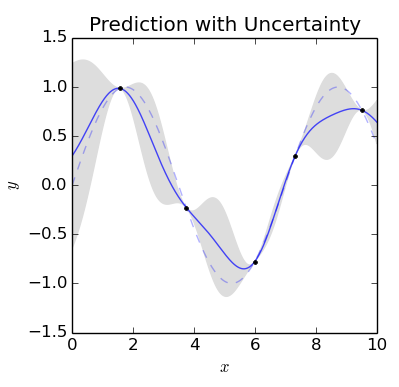
\includegraphics[width=0.4\linewidth]{Gaussian_Process_Regression.png}
	\caption{An illustration of a one-dimensional GP. The
		function used to generate the data points 
		is shown with the dashed line. The available data points are shown in
		black. The mean interpolated prediction is shown in blue
		along with the gray region showing the 68\% 
		credible interval. This figure is taken from Cdipaolo96 at 
		the Wikimedia Commons under the Creative Commons license 4.0
\label{fig:one_d_gaussian_process}}
\end{figure}
This shows the probabilistic nature of the GP predictions
(See Fig. \ref{fig:one_d_gaussian_process}).
Each drawn function represents one realization of the smoothed
field, which can be used to model the lensing potential $\psi$ later on. 
By drawing many realizations of $\psi$, we can obtain the
corresponding credible levels.
Note that the credible levels are wider for regions with less data to reflect
higher uncertainty. A GP is said to have indefinite dimension due to its ability to
predict values in unobserved regions, even though the 
observed part of the kernel is of finite size (e.g. $\ngal \times \ngal$). 
By averaging the drawn realizations, we can
obtain the mean prediction. 


When the input data is mean-subtracted, we can use a zero mean function in the
GP and the covariance kernel completely specifies the GP. 
There are several families of commonly used covariance kernel.
The ones that are of the highest interest to cosmic shear modeling 
are kernels that can capture 
the homogeneity and the isotropy of the data. This allows predicted spatial fields
$\psi$ to have consistent properties as the large-scale matter distribution.
%  Since our project wants to specify 
% The main difficulty of this project, 

The joint PDF can carry more information,
such as the uncertainties from the inputs, 
than summary statistics such as the 2PCF  



Other statistic that have been explored for capturing cosmic shear information
include aperture mass statistic $M_{\rm ap}$ or shear peak count \citep{Bard2014}.

A statistical model that makes use of the GP usually decomposes 
the signal and the noise in the following way: 
\begin{equation}
	e_{\rm obs} = g(\xv) + \epsilon_n^{\rm int}  
\end{equation}

% likelihood 
% prior 
how how  


The mean predictions from a GP are
often more well behaved and do not show drastic increase or decrease 
in the tail regions where there is no data as other polynomial interpolation schemes 
would.  



\subsection{Adapting the exponential squared kernel with lensing physics}
One of the most popular kernels that can generate homogeneous and
isotropic data is the exponential squared kernel: 
\begin{equation}
	\kerngp(r^2) = \lambda^{-1} \exp\left(\frac{-r^2}{2 l^2}\right),
	\label{eq:exp_sq_kernel}
\end{equation}
where 
\begin{equation}
	r^2 \equiv (\xv - \yv)^T \Matrix{D} (\xv - \yv), 
\end{equation}
This kernel only depends on the
squared magnitude of distances between pairs of galaxy locations. 
This chosen form is therefore invariant
under translational and rotational transformations.
The metric $\Matrix{D}$ is taken to be a diagonal matrix in this discussion but  
can be generalized to account for anamorphic distortions. 
The precision parameter $\lambda$ affects the 
amplitude of the density perturbation, while the correlation length $l^2$ 
determines how fast the correlations between different spatial locations of the
field $\psi$ fall off as a function of the spatial distance.

Additionally, the exponential squared kernel is infinitely differentiable. This
differentiable kernel choice allows us to derive an analytical expression to
relate the different lensing observables.  
In the Newtonian limit, the scalar lensing potential $\psi$ is related to 
each of the lensing observables mentioned in chapter 1, e.g. 
$\lensparams \equiv [\kappa, \gamma_1, \gamma_2]$, via the following derivatives:
\begin{align}
\kappa &= \frac{1}{2}\left(\frac{\partial^2 \psi}{\partial x_1^2} +
\frac{\partial^2 \psi}{\partial x_2^2 }\right) 
= \frac{1}{2} (\psi_{,11} + \psi_{,22}),\\ 
\gamma_1 
&=\frac{1}{2}\left(\frac{\partial^2 \psi}{\partial x_1^2} - 
\frac{\partial^2 \psi}{\partial x_2^2}\right) 
= \frac{1}{2} (\psi_{,11} - \psi_{,22}), \\
\gamma_2 
&=\frac{1}{2}\left(\frac{\partial^2 \psi}{\partial x_1 \partial
x_2} + \frac{\partial^2 \psi}{\partial x_2 \partial x_1}\right)
= \frac{1}{2} (\psi_{,12} + \psi_{,21}), 
\end{align}
where we have defined the shorthand for spatial derivatives with
subscripts for $h,i,j,k = 1, 2$ after a comma.
Since the covariance operator is linear, we can interchange the order of
operation between the covariance operator and the differentiation operator. 
The resulting 4th derivatives of the covariance
kernels $\kerngp_{\rm GP}$ have the following forms: 
\begin{align}
	\label{eq:kernel_derivatives1}
	\Cov (\kappa(\xv), \kappa(\yv))
&= \frac{1}{4}\left(
\kerngp_{,1111} + \kerngp_{,1122} + \kerngp_{,2211} + \kerngp_{,2222}
\right), \\
\Cov(\kappa(\xv), \gamma_1(\yv)) &= \frac{1}{4}\left(
\kerngp_{,1111} + \kerngp_{,2211} - \kerngp_{,1122} - \kerngp_{,2222}
\right), \\
\Cov(\kappa(\xv), \gamma_2(\yv)) &= \frac{1}{4}\left(
\kerngp_{,1112} + \kerngp_{,2212} + \kerngp_{,1121} + \kerngp_{,2221}
\right),\\
\Cov(\gamma_1(\xv), \gamma_1(\yv)) &= \frac{1}{4}\left(
\kerngp_{,1111} - \kerngp_{,1122} - \kerngp_{,2211} + \kerngp_{,2222}
\right), \\
\Cov(\gamma_1(\xv), \gamma_2(\yv)) &= \frac{1}{4}\left(
\kerngp_{,1112} + \kerngp_{,1121} - \kerngp_{,2212} - \kerngp_{,2221}
\right), \\
\Cov(\gamma_2(\xv), \gamma_2(\yv)) &= \frac{1}{4}\left(
\kerngp_{,1212} + \kerngp_{,1221} + \kerngp_{,2112} + \kerngp_{,2121}
\right),
	\label{eq:kernel_derivatives2}
\end{align}
where
\begin{equation}
	\kerngp_{,hijk} = \frac{\partial^4 \kerngp}{\partial x_h \partial x_i
	\partial y_j \partial y_k}.
\end{equation}

With the definition of ${\bf X}_i$ as follows:
\begin{equation}
	\frac{\partial r^2}{\partial \xv_i} = -\frac{\partial
	r^2}{\partial \yv_i} =
	2 \Matrix{D}(\xv - \yv)_i \equiv 2{\bf X}_i,
\end{equation}
we can show that each entry $\nu_{,hijk}$ of $\kerngp_{,hijk}$ is
related to each entry $\nu$ of the original exponential squared kernel
$\kerngp$ by:
\begin{equation}
\nu_{,x_h x_i y_j y_k} = (\beta^4 X_h X_i X_j X_k -
\beta^3 (X_h X_i \Matrix{D}_{jk} \delta_{jk} + 5~{\rm perm.}) + \beta^2
(\Matrix{D}_{hj} \Matrix{D}_{ik}\delta_{hj}\delta_{ik} + 2~{\rm perm.})) \nu,
\label{eq:4thderivatives}
\end{equation}
with $\beta = l^{-2}$. There are 6 permutations (abbreviated as perm.) of the terms in
eq. \ref{eq:4thderivatives}
multiplied to $\beta^3$ due
to choosing two pairs of indices from the $h,i,j,k$ where the order of each
pair of indices matters when we differentiate the terms by parts. 
Likewise, there are 3 possible permutations of
the terms the multiplied to $\beta^2$ due to choosing two pairs of indices from
$h, i, j, k$ where the order of the pairs does not matter.
The derivation of the relevant derivatives and terms are available 
in the appendix for completeness. 
Our implementation of the GP kernels in eqn \ref{eq:kernel_derivatives1} - 
\ref{eq:kernel_derivatives2} is openly available at
\href{https://github.com/karenyyng/george}{https://github.com/karenyyng/george}.


\subsection{Bayesian framework for inferring cosmic shear}
\begin{figure}
	\centering
	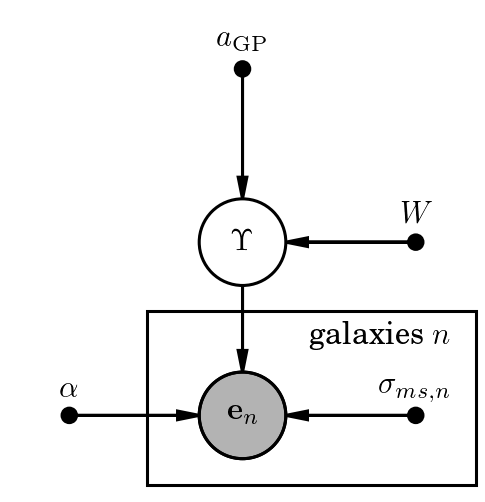
\includegraphics[width=0.4\linewidth]{shear_gp_pgm.png}
	\caption{A simplified probabilistic graphical model (pgm) for inferring
		the lensing observables $\Upsilon$ from survey or simulation data. The dots
		denote fixed parameters in the statistical procedure. The circle denotes
		latent variable, while the shaded circle denotes 
		the observed variable. The plate notation shows the galaxy entries to sum
		over.
		\label{fig:simplified_pgm}}
\end{figure}

\begin{figure}
	\centering
	\includegraphics[width=0.4\linewidth]{shear_general_pgm.png}
	\caption{A more general probabilistic graphical model (pgm) for inferring
		the lensing observables $\Upsilon$. The circle denotes
		latent variable, while the shaded circle denotes 
		the observed variable. The plate notation shows the galaxy entries to sum
		over.
		\label{fig:general_pgm}}
\end{figure}

\begin{figure}
	\centering
	\includegraphics[width=0.8\linewidth]{gp_cov_v2.png}
	\caption{An illustration of the GP covariance kernel for the data set
		presented in Schneider et al. (in prep.). The  
		\label{fig:GP_kernel_vis}}
\end{figure}




Throughout the analyses present in this work, 
we make use of the weak shear approximation 
$g = \gamma / (1 - \kappa)  \approx \gamma$, so the observed ellipticity can be
written as: 
\begin{equation}
	\epsilon_{\rm obs} = \epsilon_{\rm int} + g 
\end{equation}
assume that the shape noise term $\epsilon_{\rm int}$ of each galaxy is 
independent and follow the same Gaussian distribution.  

\subsection{Making predictions (interpolation) with a GP}
We know the joint probability density function for the observables of a GP:
\begin{equation}
	[\lensparams',\lensparams]^T \sim \mathcal{N}(0, \kerngp_{\rm GP})
\end{equation}
where we can represent the kernel matrix as several submatrices:
\begin{equation}
	\kerngp_{\rm GP} = \left[\begin{array}{cc}
	A & B \\
	B^T & C 
\end{array} \right].	
\end{equation}
We can prove that the different observations from a multivariate Gaussian are 
conditionally independent with the Schur complement:
\begin{equation}
	\mathbb{E}(\lensparams'|\lensparams) = \mathbb{E}(\lensparams) + BC^{-1}(\lensparams - \mathbb{E}(\lensparams))
\end{equation}
and
\begin{equation}
	\Cov(\lensparams'|\lensparams) = A - BC^{-1}B^T
\end{equation}
so we know how to draw new predictions $\lensparams'$ from the conditional distribution:
\begin{equation} 
	\lensparams' | \xv', \xv, \lensparams \sim \mathcal{N}(
		\mathbb{E}(\lensparams'| \lensparams), \Cov(\lensparams'|\lensparams)
	)
\end{equation}


In the presence of shape noise and measurement uncertainties, the actual 
expression of the conditional distribution used for interpolation in the actual analysis 
is slightly more complicated. But the general idea of the above derivation follows 
since we also assume the shape noise and the measurement uncertainties to be Gaussian.
Similarly, once we can find GP parameters $\gpparams$ that can allow us to fit
the observed shear fields $\gamma_{(1, 2)}$ at $\xv$, we can compute $\kerngp_{(\kappa,
\kappa)}$ and draw predictions for $\kappa$ from the conditional distribution. 

\subsection{The computational performance of our method}
We implemented the covariance kernels in \ref{eq:kernel_derivatives1}
via {\sc C++} along with a {\sc Python} wrapper. 
Although the operation of computing and assembling the
derivatives are $O(\ngal^2)$, the large number of addition and 
multiplication operations can be slow.
Exploiting the symmetry of the covariance kernel can only provide 
memory saving of a factor of 2.
To speed up the computation to make it feasible, 
I implemented the parallelized computation of each element of the kernel using 
the {\sc OpenMP} library. The slowest step of the entire computation, however, 
is the inversion of the
covariance kernel matrix for the evaluation of the marginal likelihood, 
which is an $O(\ngal^3)$ operation. 
I made use of a parallelized version of the Cholesky decomposition via the {\sc Intel Math
Kernel Library} to invert the matrix and achieved $\sim10$ 
times speed up so the
computation and the evaluation of the likelihood of each set of GP parameter
take $< 10s$ for 1600 galaxies, which translates to 
the inversion of a 4200 $\times$ 4200 covariance matrix.
With the use of distributed computational resources, it is possible 
to probe the space of possible GP parameters.  

\section{Results}
 \begin{figure}
	\centering
	\includegraphics[width=0.7\linewidth]{mass_map_comparison_galsim.png}
	\caption{A comparison of mass maps for simulated inputs from {\sc GalSim} and
	the mass map generated with the use of a GP prior \label{fig:Galsim_massmaps}. 
	This figure is part of Schneider et al. (in prep.).
}
\end{figure}

\begin{figure}
	\centering
	\includegraphics[width=0.4\linewidth]{kappa_Abell781.png}
	\includegraphics[width=0.4\linewidth]{kappa_Abell781_WD.png}
	\caption{A comparison of mass maps for Abell 781 in the Deep Lens Survey (DLS) 
		\label{fig:Abell781_massmap}.  Left: The smoothed mass map of Abell 781 from 
		Right: The output generated with 6000
		galaxies. 
	These figures are part of Schneider et al. (in prep.).
}
\end{figure}



\begin{table}%[htb]
% \small
\begin{center}
\caption{Parameters for the statistical model.}
\label{tab:sampling_parameters}
\begin{tabular}{cl}
\hline
Parameter & Description \\
\hline
${\bf d_{n}}$ & data vector (measured $e_{1,2}$ for each galaxy $n$)  \\
$\sigma_{{\rm ms}; n}$ & ellipticity measurement error for galaxy $n$ 
\\
$\xv$, $\yv$ & vector(s) of 2D spatial locations of galaxies \\
$\epsilon_n^{\rm int}$ & intrinsic galaxy ellipticity for galaxy $n$ \\
$\alpha\equiv\sigma_{e}^2$ & parameters of the distribution of galaxy parameters \\
W & window function for the survey footprint \\
$\lensparams$ & lensing shear and convergence ($\gamma_{1,2}, \kappa$) \\
$\gpparams$ & parameters of the GP kernel\\
% $\rho_{\rm GP}$ & correlation of the GP kernel (element of $\gpparams$) \\
$\lambda$ & precision of the GP kernel (element of $\gpparams$) \\
$l^2$ & squared GP correlation length (element of $\gpparams$) \\
% $\lambda_{\epsilon}$ & precision for the nugget term (element of $\gpparams$) \\
\hline
\end{tabular}
\end{center}
\end{table}



\subsection{Verification using {\sc GalSim} simulated data}
\subsection{Mass mapping for Deep Lens Survey Abell 781}

% Is a non-trivial optimization problem 

\section{Discussion}

\subsection{Relating the lensing observables to a cosmological model}
We can draw realizations of the lensing observables from the GP given a set of
optimized GP parameters:
\begin{equation}
	\lensparams(\xv) \sim GP(0, \kerngp_{\rm GP}(\xv, \yv)) 
\end{equation}


The constraints on cosmological parameters need to be verified in a mock
weak-lensing analysis of cosmological simulation. 
It can enable the separation of E and B mode in the convergence field as shown
in Schneider et al. (in prep.) 

\subsection{Use of the Gaussian Process in the model fitting for shear}
We describe a simplified graphical model to demonstrate how the derived GP can
be used to infer cosmic shear and a mass map from the convergence.
A more sophisticated model can be found in Schneider et al. 2016.



% - [ ] TODO add PGM 
% talk about the lensing approximations that were made 


% \subsection{Sampling grid and the correlation length}
% A weakness of the method is the apparent reliance on having the sampling 

\subsection{Alternative kernel choice(s) for encoding the lensing physics}
Alternative choices for a covariance kernel for describing the lensing physics 
include the family of Mat\'{e}rn kernels:
% \begin{equation}
% 
% \end{equation}

The smoothness of the data generated from a Mat\'{e}rn kernel is closely
related to the degree of freedom of the kernel. 
The higher degree of freedom it has, the smoother the spatial variations of the
drawn $\psi$ would be for the same correlation length.
Note that a Mat\'{e}rn kernel is also only differentiable to the $i$-th order,
where $i$ is [TODO] related to the degree of freedom by [TODO].
This restricts us to use kernels with degree of freedom above [TODO]. 
When we take the limit of the degree of freedom of a Mat\'{e}rn kernel to infinity, 
we recover the exponential squared kernel.

It is possible to generalize the derivation of derivatives by using automatic
differentiation. Automatic differentiation may allow evaluation of other
kernels that generates isotropic and homogeneous data, 
such as the Mat\'{e}rn kernels.  
% An implementation via numerical differentiation may
% or may not be more computationally intensive to
% compute, depending on the required numerical precision (aka order of accuracy).
Differentiation technology such as automatic differentiation, 
that spreads factors of the derivatives over a tree like structure for
almost exact computation can be considered, but is outside the scope of this work.



\subsection{Possible separation of the E / B mode}

% - [ ] describe why the lensing observables shouldn't have a B mode 

It is not obvious what kernel choices will allow one to capture the B-mode 
in the data.
We can separate the E and the B mode of the shear, those derivation can be seen in  
\cite{Schneider2001a}.
 \begin{align}
	\kappa^E & = \kappa\\
	\kappa^B & = 0 \\
	\gamma^E &= \left[\frac{1}{2} (\psi^E_{,11} - \psi^E_{,22}) -
	\psi^B_{,12}\right]\\
	\gamma^B &= \left[\psi^E_{,12} + \frac{1}{2} (\psi^B_{,11} - \psi^B_{,22})\right]
\end{align}


\subsection{Modeling systematics and noise}
Besides kernels that describes homogeneous and isotropic data,
there are other types of periodic kernels that may be useful
in modeling systematics such as masking or footprints of chip gaps due to the
stacking of multiple exposures.
For spatial models with undetermined periodicity or patterns, 
composite kernels with different covariance structures 
can be formed by the addition and/or multiplication of several kernels
 to pick up (sometimes non-obvious) patterns in the data. 
A GP with composite kernels is a
famous example how both the short-and-long term trends of global carbon
dioxide level can be modeled and predicted \citep{Duvenaud2013}.



% Can handle sharp boundaries from stacking images 
% cite Jee2013a  
% cite Rowe2010 paper for interpolating star fields for 
% PSF ellipticity corrections 

\subsection{Speeding up the matrix operations}
Currently, our method is not as computationally competitive as the 2PCF. One of
the fastest implementation has a computational complexity of $O(N\sqrt{N})$.
The 2PCF algorithm has also been demonstrated to scale well with a distributed and parallelized
implementation \citep{Chhugani2012}.

Rather than relying on manual intensive methods for parallelizing the
computation of the kernel methods, a more promising way is to approximate the
small elements in the covariance kernel structure as zero. 

The relevant field of literature about how approximating the kernel as a sparse
matrix may affect the
statistical inference is called covariance tapering. 
On the other hand, \citep{Snelson2006}
there are papers demonstrating that synthetic data with much less data points  
would produce further 
With large amount of
sparsity, the inversion of the matrix can be sped up to [TODO]$O(M^2N)$ for
building the model and $O(M^2)$ for interpolating / predicting output functions
at new input locations \citep{Snelson2006}.
  

\section{Conclusion}
Here, we have derived and implemented a fully probabilistic method for 
representing the lensing observables. It can potentially  

The potential of using a Gaussian Process for the inference of cosmological 
Gaussian Process (GP)parameters remains to be proved. 

Requires the understanding of the underlying physical observable, how the statistical
approach can carry the information and how to actual execute the computation in
a tractable way.


\section{Acknowledgement}
We thank Chris Paciorek for discussion about the statistical
framework for performing shear inference and the
use of Gaussian Processes.
This research
used the resources of the National Energy Research Scientific 
Computing Center (NERSC), a DOE Office of Science
User Facility supported by 
of the U.S. Department of Energy under Contract No.
DE-AC02-05CH11231.
 This work uses a modified version
of the public code {\sc George} available at \href{https://
github.com/karenyyng/george}{https://
github.com/karenyyng/george}, which was forked from \\
\href{https://github.com/dfm/george}{https://github.com/dfm/george}.



\appendix 

\section{Derivation of GP kernel}


\subsection{The relevant 4th spatial derivatives}
We show how to derive one of the 6  covariance matrices that we can compute
from $\lensparams = [\kappa, \gamma_1, \gamma_2]$. The computation of the other
covariance kernels is completely analogous.
\begin{align*}
&{\rm Cov}_{m,n} (\kappa(\vec{x}), \kappa(\vec{y}))  \\ 
&= \mathbb{E} \left[ 
	(\kappa - \mathbb{E}[\kappa])|_m 
( \kappa - \mathbb{E}[\kappa])|_n\right] 
\\
 &=\mathbb{E}\left[
\frac{1}{2} \left(\frac{\partial^2}{\partial y_1^2} + 
\frac{\partial^2}{\partial y_2^2}\right) 
 (\psi - \mathbb{E}\left[\psi\right])|_n \frac{1}{2}
\left(\frac{\partial^2}{\partial x_1^2} + \frac{\partial^2}{\partial x_2^2} \right)
(\psi - \mathbb{E}\left[\psi\right])|_m \right]
\\
&= \frac{1}{4}\left(
\frac{\partial^2}{\partial x_1^2} \frac{\partial^2}{\partial y_1^2} + 
\frac{\partial^2}{\partial x_1^2} \frac{\partial^2}{\partial y_2^2} +  
\frac{\partial^2}{\partial x_2^2} \frac{\partial^2}{\partial y_1^2} + 
\frac{\partial^2}{\partial x_2^2} \frac{\partial^2}{\partial y_2^2}  
\right) \kerngp_{mn}\\ 
\end{align*}


\subsection{The actual terms from the 4th derivatives}
\begin{equation*}
\kerngp = \lambda^{-1} \Sigma 
\end{equation*}

\begin{align}
\Sigma &= \exp{\left(\frac{-\beta}{2} r^2 \right)}\\
\Sigma_{,x_i} &= \frac{-\beta}{2} \Sigma r^2_{,x_i} = -\beta \Sigma X_i\\ 
\Sigma_{,y_h} &= \beta \Sigma X_h 
\end{align}

\begin{align}
\Sigma_{,x_i x_j} &= \frac{-\beta}{2}(\Sigma_{,x_j} r^2_{,x_i} + \Sigma r^2_{,x_i x_j})\\
\Sigma_{,x_i x_j y_h} &= \frac{-\beta}{2}(\Sigma_{,x_j y_h} r^2_{,x_i} + \Sigma_{,x_j}
r^2_{,x_i y_h} + \Sigma_{,y_h} r^2_{,x_i x_j})\\
\Sigma_{,x_i x_j y_h y_k} &= \frac{-\beta}{2} 
(\Sigma_{,x_j y_h y_k} r^2_{,x_i} +
\Sigma_{,x_j y_h} r^2_{,x_i y_k} + 
\Sigma_{,x_j y_k} r^2_{,x_i y_h} + 
\Sigma_{,y_h y_k} r^2_{,x_i x_j} )
\label{eq:4th_derivative_intermediate_expression}
\end{align}

Just work on terms that are parts of the 4th kernel derivative 
\begin{align*}
\Sigma_{,x_i x_j} &= \frac{\partial}{\partial x_j} (-\beta \Sigma X_i)\\
&= -\beta(\Sigma_{,x_j X_i} + \Sigma X_{i, x_j})\\ 
&= -\beta(-\beta \Sigma X_j X_i + \Sigma \delta_{ij} \mathsf{D}_{ij}) \\ 
&= (\beta^2 X_j X_i - \beta \delta_{ij} \mathsf{D}_{ij})\Sigma 
\end{align*}

\begin{align*}
\Sigma_{,x_i y_h} &= \frac{\partial}{\partial y_h} (-\beta \Sigma X_i)\\
&= -\beta(\Sigma_{,y_h X_i} + \Sigma X_{i, y_h})\\ 
&= -\beta(\beta \Sigma X_h X_i - \Sigma \delta_{ih} \mathsf{D}_{ih}) \\ 
&= -(\beta^2 X_h X_i - \beta \delta_{ih} \mathsf{D}_{ih})\Sigma 
\end{align*}

\begin{align*}
\Sigma_{,y_h y_k} &= \frac{\partial}{\partial y_h} (\beta \Sigma X_h)\\
&= \beta(\Sigma_{,y_k X_h} + \Sigma X_{h, y_k})\\ 
&= \beta(\beta \Sigma X_k X_h - \Sigma \delta_{hk} \mathsf{D}_{hk}) \\ 
&= (\beta^2 X_h X_k - \beta \delta_{hk} \mathsf{D}_{hk})\Sigma 
\end{align*}

\begin{align}
\Sigma_{,x_i x_j} &= (\beta^2 X_j X_i - \beta \delta_{ij} \mathsf{D}_{ij})\Sigma\\ 
\Sigma_{,x_i y_h} &= -(\beta^2 X_h X_i - \beta \delta_{ih} \mathsf{D}_{ih})\Sigma\\ 
\Sigma_{,y_h y_k} &= (\beta^2 X_h X_k - \beta \delta_{hk} \mathsf{D}_{hk})\Sigma 
\end{align}

Term 1 of the 4th derivative of eqn \ref{eq:4th_derivative_intermediate_expression}

\begin{align*}
\Sigma_{,x_j y_h y_k}
&= \frac{\partial}{\partial y_k} \Sigma_{,x_j y_h}\\ 
&= -\frac{\partial}{\partial y_k} (\beta^2 X_h X_j - \beta \delta_{jh} \mathsf{D}_{jh})\Sigma\\
&= (\beta^2 \mathsf{D}_{hk} \delta_{hk} X_j + \beta^2 X_h \mathsf{D}_{jk}\delta_{jk})\Sigma -
(\beta^2 X_h X_j - \beta \mathsf{D}_{jh} \delta_{jh})\beta X_k \Sigma
\end{align*}

\begin{align*}
&\Sigma_{,x_j y_h y_k} r_{,x_i}^2\\
&= 2[\beta^2 X_j \mathsf{D}_{hk} \delta_{hk} + \beta^2 X_h \mathsf{D}_{jk}\delta_{jk} +
\beta^2 X_k \mathsf{D}_{jh} \delta_{jh} - \beta^3 X_h X_j X_k] X_i \Sigma\\ 
&=\boxed{2\beta^2[ 
X_j X_i \mathsf{D}_{hk} \delta_{hk} + 
X_h X_i \mathsf{D}_{jk} \delta_{jk} + 
X_k X_i \mathsf{D}_{jh} \delta_{jh}] \Sigma 
- 2\beta^3 X_h X_j X_k X_i \Sigma} 
\end{align*}

\subsection{Term 2 of the 4th derivative}
\begin{align*}
\Sigma_{,x_j y_h} r^2_{,x_i y_k}
&= - (\beta^2 X_h X_j - \beta \mathsf{D}_{jh} \delta_{jh}) (-2\mathsf{D}_{ik}
\delta_{ik} \Sigma) \\  
&= \boxed{( 2 \beta^2  X_h X_j \mathsf{D}_{ik} \delta_{ik} 
-2 \beta \mathsf{D}_{jh} \mathsf{D}_{ik} \delta_{jh} \delta_{ik}) \Sigma} 
\end{align*}

\subsection{Term 3 of the 4th derivative}
This is completely analogous to term 2 except the subscripts are slightly
different
\begin{align*}
\Sigma_{,x_j y_k} r^2_{,x_i y_h}
&=\boxed { ( 2 \beta^2  X_k X_j \mathsf{D}_{ih} \delta_{ih} 
-2 \beta \mathsf{D}_{jk} \mathsf{D}_{ih} \delta_{jk} \delta_{ih}) \Sigma} 
\end{align*}

\subsection{Term 4 of the 4th derivative} 
\begin{align*}
\Sigma_{,y_h y_k} r^2_{,x_i x_j}
&= (\beta^2 X_k X_h - \beta \mathsf{D}_{hk}\delta_{hk})\Sigma 2 \mathsf{D}_{ij} \delta_{ij}\\ 
&= \boxed{(2\beta^2 X_k X_h \mathsf{D}_{ij} \delta_{ij} - 2\beta \mathsf{D}_{ij} \mathsf{D}_{hk} \delta_{hk}
\delta_{ij})\Sigma } 
\end{align*}

Collecting terms of $\Sigma_{,x_i x_j y_h y_k}$ by plugging them in eqn
\ref{eq:4th_derivative_intermediate_expression}
, we have 
\begin{align}
\nu_{,x_i x_j y_h y_k} &= (\beta^4 X_h X_j X_k X_i -  
\beta^3 (X_j X_i \mathsf{D}_{hk} \delta_{hk} + 5 {\rm perm.}) + \beta^2
(\mathsf{D}_{jh} \mathsf{D}_{ik}\delta_{jh}\delta_{ik} + 2 {\rm perm.})) \nu \\
&= \gamma \nu
\end{align}

Where $\nu$ is an entry in the matrix $\Sigma$


	% The following commands produce page numbering at the bottom
% center using roman numerals per UC Davis requirements for the
% front matter of the dissertation:
% \pagenumbering{roman}
% \pagestyle{plain}
% The following command produces double-spaced lines for the
% remainder of the document:
\doublespacing

\setcounter{chapter}{4}
\chapter{Conclusion}{}{}
\label{chapter5}




	% -- Appendix 1
	\appendix
	
% The following commands produce page numbering at the bottom
% center using roman numerals per UC Davis requirements for the
% front matter of the dissertation:
% \pagenumbering{roman}
% \pagestyle{plain}
% The following command produces double-spaced lines for the
% remainder of the document:
\doublespacing
\chapter{Supplementary material of the study of El Gordo}{}{}
\label{appendix1}

				 
% % \cfoot{\thepage}
% % \pagenumbering{arabic}
% 
% \section{Default weights used for Dawson's Monte Carlo simulation}
% \label{app:priors}
% The default weight that we employed can be summarized as
% follows for most of the output variables: 
% \begin{equation}
% 	w(v_{3D}(t_{\rm per})) = 0\text{ if }v_{3D}(t_{\rm per}) >
% 	v_{\text{free fall}}. 
% \end{equation}
% \begin{equation}
% 	w(TSP_{\rm out}) = 
% 	\begin{cases}
% 		& \text{const}~\text{if }TSP_{\rm out} < \text{age of universe at } z=0.87	\\
% 		& 0~\text{otherwise}.
% 	\end{cases}
% \end{equation}
% In addition, we apply the following weight on $TSP_{\rm ret}$:
% \begin{equation}
% 	w(TSP_{\rm ret}) = 
% 	\begin{cases}
% 		& \text{const}~\text{if }TSP_{\rm ret} < \text{age of universe at } z=0.87	\\
% 		& 0~\text{otherwise} \label{eqn:TSM_1}.
% 	\end{cases}
% \end{equation}
% To correct for observational limitations, we further convolved the
% posterior probabilities of the different realizations with 
% \begin{equation}
% 	w(TSP_{\rm out} | T) = 2 \frac{TSP_{\rm out}}{T},
% \end{equation}
% to account for how the subclusters move faster at lower $TSP$ and thus it
% is more probable to observe the subclusters at a stage with a larger $TSP$.
% \par 
% \section{Plots of outputs of the Monte Carlo simulation}
% We present the PDFs of the inputs of the dynamical simulation and the
% marginalized PDFs of the outputs after applying the polarization weight in
% addition to the default weights. See Fig.~\ref{fig:plot_config} for explanations of
% the order that we present the figures containing the PDFs . 
% \begin{figure}
% 	\begin{center}
% 	\includegraphics[width=\linewidth]{ElGordo_plot_config.png}
% 	\end{center}
% 	\caption{Matrix of variables used in the simulations. We present them in
% 	4 categories, including, inputs, geometry, time and velocity. Regions of
% 	the same color represent one plot and the number
% indicates the corresponding figure number in this appendix.
% \label{fig:plot_config}
% }
% \end{figure}
% \label{app:results}
% %%%%%%%%%%%%% TASK --- 
% \clearpage
% \begin{figure*}
% 	\begin{minipage}{180mm}
% 	\begin{center}
% 	\includegraphics[width=0.65\linewidth]{TwoMnWBSG_inputsVsinput.png}
% 	\caption{Marginalized 2-dimensional PDFs of original inputs (vertical axis) 
% 		and the inputs after applying polarization weight and default weights 
% 		(horizontal axis). The inner and outer contour
% denote the central 68\% and 95\% confidence regions respectively.
% The circular contours show that the application of weights did not introduce
% uneven sampling of inputs. }
% 	\end{center}
% 	\end{minipage}
% \end{figure*}
% \begin{figure*}
% \begin{minipage}{180mm}
% 	\begin{center}
% 	\includegraphics[width=0.5\linewidth]{TwoMnWBSG_tri_geo.png}
% 	\caption{One-dimensional marginalized PDFs (panels on the diagonal) and
% 		two-dimensional marginalized PDFs of variables
% 		denoting characteristic distances and projection angle of the mergers.
% 	\label{fig:geom_geom}
% 	}
% 	\end{center}
% 	\end{minipage}
% \end{figure*}
% \begin{figure*}
% \begin{minipage}{180mm}
% 	\begin{center}
% 	\includegraphics[width=0.7\linewidth]{TwoMnWBSG_geoVSinputs.png}
% 	\caption{Marginalized PDFs of characteristic distances and projection
% 		angle of the merger and the inputs of the simulation.}
% 	\end{center}
% 	\end{minipage}
% \end{figure*}
% \begin{figure*}
% \begin{minipage}{180mm}
% 	\begin{center}
% 	\includegraphics[width=0.5\linewidth]{TwoMnWBSG_tri_time.png}
% 	\caption{One-dimensional PDFs of characteristic timescales of the simulation
% (panels on the diagonal) and the marginalized PDFs of different
% timescales. Note that there is a default weight for constraining $TSP_{\rm out}$ but
% not for $TSP_{\rm ret}$ and $T$, so $TSP_{\rm out}$ spans a smaller range.}
% 	\end{center}
% \end{minipage}
% \end{figure*}
% \begin{figure*}
% \begin{minipage}{180mm}
% 	\begin{center}
% 	\includegraphics[width=0.5\linewidth]{TwoMnWBSG_timeVsgeo.png}
% 	\caption{Marginalized PDFs of characteristic timescales of the simulation
% and the characteristic distances and the projection angle of the merger. }
% 	\end{center}
% \end{minipage}
% \end{figure*}
% \begin{figure*}
% \begin{minipage}{180mm}
% 	\begin{center}
% 	\includegraphics[width=0.7\linewidth]{TwoMnWBSG_timeVSinput.png}
% 	\caption{Marginalized PDFs of characteristic timescales of the simulation
% and the inputs.}
% 	\end{center}
% \end{minipage}
% \end{figure*}
% \begin{figure*}
% \begin{minipage}{180mm}
% 	\begin{center}
% 	\includegraphics[width=0.5\linewidth]{TwoMnWBSG_tri_vel.png}
% 	\caption{One-dimensional marginalized PDFs of velocities at
% 	characteristic times (panels on the diagonal) and marginalized PDFs of
% different velocities.}
% 	\end{center}
% \end{minipage}
% \end{figure*}
% \begin{figure*}
% \begin{minipage}{180mm}
% 	\begin{center}
% 	\includegraphics[width=0.5\linewidth]{TwoMnWBSG_velVStime.png}
% 	\caption{Marginalized PDFs velocities and the characteristic timescales
% 	of the simulation against the inputs.}
% 	\end{center}
% \end{minipage}
% \end{figure*}
% \begin{figure*}
% \begin{minipage}{180mm}
% 	\begin{center}
% 	\includegraphics[width=0.5\linewidth]{TwoMnWBSG_velVSgeo.png}
% 	\caption{Marginalized PDFs of the velocities at characteristic timescales
% 		and the characteristic distances and the projection angle of the merger. }
% 	\end{center}
% \end{minipage}
% \end{figure*}
% \begin{figure*}
% \begin{minipage}{180mm}
% 	\begin{center}
% 	\includegraphics[width=0.7\linewidth]{TwoMnWBSG_velVSinputs.png}
% 	\caption{Marginalized PDFs of relative velocities characteristic
% 	timescales of the simulation and the inputs.}
% 	\end{center}
% \end{minipage}
% \end{figure*}
% 
% \section{Comparison of the outgoing and returning scenario}
% \label{app:Bayes_factor}
% Here, we compare the different merger scenarios using the two relics
% independently and show that they consistently give the conclusion that the returning
% scenario is favored for the plausible range of $\beta$. For each merger
% scenario, we compute
% the (marginalized) probability of producing simulated
% values ($s_{proj}$) compatible with the observed location of the radio
% relic ($s_{obs}$). 
% 
% Quantitatively, we want to compute and compare the probability:  
% \begin{align} 
% 	&P(s_{proj} \text{ compatible with }s_{obs} | M)  \label{eqn:prob}\\
% 	&=\iint f(S_{proj} \cap S_{obs} | M, \beta) f(\beta | M) d s_{proj} d\beta\\
% 	&=\iint  f(s_{proj}|M, \beta) f(s_{obs}) f(\beta | M) d s_{proj}
% 	d\beta, 
% \end{align}
% where $f$ indicates the corresponding PDF, $M$
% represents one of the merger scenarios, and $\beta$ is defined in equation
% ~\ref{eqn:NW_speed}, $s_{proj} \in S_{proj}$ and $s_{obs} \in S_{obs}$. 
% We set our priors set to be uniform for the marginalization: 
% \begin{equation}
% 	f(\beta | M_{ret}) = f(\beta | M_{out}) =  
% 	\begin{cases}
% 		& \text{const}~\text{if } 0.7 \leq \beta \leq 1.5 \\
% 		& 0~\text{otherwise}.
% 	\end{cases}
% \end{equation}
% which is more conservative than the most likely range of $\beta$, which is
% $0.7 < \beta < 1.1$.
% We found: 
% \begin{align}
% 	&P(S_{proj} \cap S_{obs} | M_{ret}) / P(S_{proj} \cap S_{obs} |
% 	M_{out})\\
% 	&=
%  \begin{cases}
% 	2.1 \text{ for the NW relic},\\
% 	460 \text{ for the SE relic},
%  \end{cases}
% \end{align}
% which shows that the returning scenario is favored over the outgoing
% scenario. 
% 
% This test quantity differs from the traditional hypothesis testing or model comparison in several ways: 
% \begin{enumerate}
% \item we did not compute a likelihood function.  We have adopted
% non-parametric PDFs in our Monte Carlo simulation,i.e. there is no well-known
% functional form of the likelihood in our context. We make use of
% $f(S_{proj} \cap S_{obs})$ to penalize the simulated values being different from our observed data
% \item with this quantity, we are not asking whether the expected value of
% 	the radio relic such as the mean or median from each model match the
% 	observation best. Those estimators take into account the values that do not match the observed location of the radio relic. 
% \item we marginalized the uncertainty in $\beta$ to be as conservative
% 	as possible, instead of assuming a fixed value of $\beta$.
% \end{enumerate} \par
% %The second quantity that we compute is the Wald statistic at a range of possible $\beta$ values.
% %Wald statistic is usually used hypothesis testing.
% %Computing the Wald statisic allows us to ask, given a particular model (merger
% %scenario),
% %whether the null value (sample mean) is in the confidence
% %interval \citep{Wasserman04}. The Wald statistic that we compute for each model is: 
% %\begin{align}
% %	W(\beta) = \frac{\bar{s}_{obs} - \mu(\beta)}{\sigma / (n)^{1/2}} 
% %\end{align}
% %where $\bar{x}$ is the sample mean, $\mu(\beta)$, $\sigma$ and $n$ are the
% %population mean, population standard deviation and size of samples of the
% %simulated model respectively. A higher Wald statistic value would represent
% %a larger difference between the observed and model value, while taking into account the model uncertainty. Within the range of
% %most likely $0.7 < \beta < 1.5$, the Wald statistic shows that the observed
% %relic location is more compatible with the confidence interval of the returning
% %scenario. (See Figure~\ref{fig:waldtest})
% 
% \begin{figure}
% 	\includegraphics[width=\linewidth]{prob_ratio.png}
% 	\caption{Probability ratio between the returning model (numerator) and
% 		the outgoing model at given $\beta$. We remind readers $\beta$ is a factor
% 		relating the {\it time-averaged} shock velocity and the pericenter
% 		velocity of the corresponding subcluster.  
% 	\label{fig:prob_ratio}}
% \end{figure}
% 
% \begin{figure}
% 	\begin{center}
% 	\includegraphics[width=0.8\linewidth]{polar_prior_bounds_E.pdf}
% 		\caption{Comparison of the PDFs of the observed position of the SE relic (red bar
% 			includes 95\% confidence interval of location of relic in the center of
% 			mass frame) with the predicted position from the two simulated merger scenarios (blue for outgoing and green for the returning scenario). 
% 		For the plausible values of $\beta < 1.1$, the returning scenario is preferred. 
% 		We obtained similar conclusion about the merger scenario as for the NW
% 		relic calculation.
% 		\label{fig:positionprior_SE}}
% \end{center}
% \end{figure}
% 
% \begin{figure}
% 	\begin{center}
% 	\includegraphics[width=.8\linewidth]{polar_prior_bounds.pdf}
% 	\caption{Comparison of the PDFs of the observed position of the NW relic (red bar
% 		includes 95\% confidence interval of location of relic in the center of
% 		mass frame) with the	predicted position from the two simulated merger scenarios (blue for outgoing and green for the returning scenario). 
% 	For the plausible values of $\beta  < 1.1$, the returning model is
% 	preferred. For comparison purpose, we also show that $\beta > 1.3$ (top
% 	panel) for the outgoing scenario to be favored.  
% 	Note that we made use of the polarization weight for producing this figure. 
% 	\label{fig:positionprior}}
% \end{center}
% \end{figure}
% \clearpage
% \section{Acknowledgements}
% We thank Franco Vazza, Marcus Br\"{u}ggen and Surajit Paul for sharing
% their knowledge on the simulated properties of radio relic and merger
% shocks. We extend our gratitude to Reinout Van Weeren for first proposing the use of
% radio relic to weight the Monte Carlo realizations. We appreciate the
% comments from Maru\v{s}a Brada\v{c} about using the position of the relic to
% break degeneracy of the merger scenario. KN is grateful to Paul Baines and
% Tom Loredo for discussion of the use of prior information and sensitivity tests. 
% Part of this work was performed under the auspices of the U.S. DOE by LLNL
% under Contract DE-AC52-07NA27344. 
% JPH gratefully acknowledges support from Chandra (grant number GO2-13156X)
% and Hubble (grant number HST-GO-12755.01-A).
% We would also like to thank 
% GitHub for providing free repository for version control for our data and
% analyses. This research made use of APLpy, an open-source plotting package for Python
% hosted at http://aplpy.github.com; Astropy, a community-developed core
% Python package for Astronomy \citep{astropy}; AstroML, a
% machine learning library for astrophysics \citep{VanderPlas2012}, and IPython, a system for
% interactive scientific computing, computing in science and engineering
% \citep{Perez2007}.\par
% Note: The authors have made the Python code for most of the analyses openly
% available at
% \href{https://github.com/karenyyng/ElGordo\_paper1}{https://github.com/karenyyng/ElGordo\_paper1}. 

	/Users/karenyng/Documents/illustris_analysis/paper/illustris_appendix.tex
	\section{Algorithm of the Shrinking aperture estimates}
\label{app:shrink_apert}
\begin{algorithm}
	\caption{Shrinking aperture algorithm with luminosity weights}
	\KwData{subhalo that satisfy cuts as a galaxy}
	 \hrulefill \\

	 initial aperture centroid = weighted mean galaxy location in each spatial dimension\\
 	distance array = euclidean distances between initial aperture center and each galaxy
	location \\
 	aperture radius = 90th percentile of the weighted distance array\\ 
	\While{ (newCenterDist - oldCenterDist) / oldCenterDist $\geq$ 2e-2}{
 		new data array = old data array within aperture\\
 		newCenter = weighted mean value of new data along each spatial dimension 
	}   \hrulefill
\end{algorithm}
\begin{figure*}
	\begin{center}
	\includegraphics[width=0.7\linewidth]{Mass_abundance_relationship.pdf}
	\caption{Cumulative distribution of clusters above a certain mass threshold
		for different samples.
		Each distribution is normalized to the sample size.
		The unrelaxed samples $1.2 < \nu < 2.2$ 
		If the subsets have the same cluster mass abundance as the full sample,
		the three plots should lie on top of one another.
		\label{fig:mass_abundance_distribution}
	}
\end{center}
\end{figure*}
 

\section{Table of results}
\label{app:table_of_results}
\begin{table}
	\begin{center}
	\ifthenelse{\boolean{thesis}}{
	\caption{Properties of the clusters used in the analysis. Richness is
	computed based on $i-$band $< 24.4$ assuming $z=0.3$.\label{tab:cluster_prop}
		The table is too large to be included inside the dissertation and is instead
	available at \href{https://goo.gl/uGUhec}{https://goo.gl/uGUhec}}
}{
	\caption{Properties of the clusters used in the analysis. Richness is
	computed based on $i-$band $< 24.4$ assuming $z=0.3$.\label{tab:cluster_prop}
}
}
\end{center}
\end{table}



\begin{landscape}
\begin{table*}
	\begin{center}
	\caption{Summary statistic characterizing the offset distributions
		between the most bound particle and various summary statistics of 
		the member galaxy population. There are explanations of the outliers in
		this table in the result subsection \ref{subsec:galaxyDMoffset}.
	\label{tab:most_bound_particle_offset_distributions}}
	\input{Chapters/most_bound_particle_table.tex}
\end{center}
\small{The offsets represented with the prime $'$ symbols are estimated using the luminosity weighted galaxy 
data.}
\end{table*}
\end{landscape}


\begin{table}
	\begin{center}
	\caption{Summary statistic characterizing the offset distributions
		for between the DM peak and the estimated galaxy location. 
		All 43 clusters and all 768 projections are used in this table. 
		The highest density values were used for the computation when there were more
		than one peak value estimated from the KDE. There are different levels of 
		asymmetry depending on how sparse a region is. 
	\label{tab:offset_distributions}}
	\input{Chapters/full_sum_stat_table}
\end{center}
\small{The offsets represented with the prime $'$ symbols are estimated using the luminosity weighted galaxy 
data.}
\end{table}




	\addcontentsline{toc}{chapter}{References}
	{\singlespacing
	\bibliography{./Chapters/chapter1,./Chapters/chapter2,./Chapters/chapter3,./Chapters/Rpackage.bib}
	}

\end{document}
